\documentclass[a4paper,12pt]{report}

\usepackage{tabularx}
\usepackage{alltt, fancyvrb, url}
\usepackage{graphicx}
\usepackage[utf8]{inputenc}
\usepackage{float}
\usepackage{hyperref}
\usepackage{caption}
\usepackage{listings}
\usepackage{xcolor}


% Questo commentalo se vuoi scrivere in inglese.
\usepackage[italian]{babel}

\usepackage[italian]{cleveref}

% Centra verticalmente i contenuti delle righe
\renewcommand\tabularxcolumn[1]{m{#1}}


\title{\textbf{Elaborato per il corso Basi di dati}
Progettazione di una base di dati per la gestione di video perizie}


\author{
\\Buizo Manuel
\\Matteini Mattia
\\Paganelli Alberto
}
\date{\today}


\begin{document}

\maketitle

\tableofcontents

\chapter{Analisi dei requisiti}

Si vuole realizzare un database a supporto della gestione di video perizie (perizie a distanza tramite videochiamata) effettuate per varie assicurazioni italiane.
\\
La base di dati dovrà immagazzinare informazioni relative a tutto l’ambito assicurativo, dalle assicurazioni, agli studi peritali che effettueranno le perizie.
\\
Si dovrà tenere conto anche di polizze, assicurati, dipendenti, documenti relativi alle video-perizie.


\section{Intervista}

Si vuole tenere traccia di tutte le video-perizie effettuate, di ogni studio peritale e delle parti coinvolte. 
\\
Ogni assicurazione genererà sinistri di varia natura (R.C.A., Furto, Incendio, ecc…).
\\
Gli assicurati stipuleranno dei contratti (polizze) con le agenzie assicurative, queste potranno essere di diversi tipi e avranno un numero identificativo, un costo, un massimale e una data di scadenza.
\\
Le assicurazioni avranno una propria denominazione e metteranno a disposizione un numero verde, una email e un numero di telefono per i contatti.
\\
Tutti i sinistri generati verranno assegnati a vari studi i quali si occuperanno di portare a termine le attività peritali. Per ogni sinistro dovremo tenere traccia del luogo dov’è avvenuto, della descrizione del danno e di quando si è verificato, inoltre sarà specificato da una categoria.
Il sinistro dovrà essere sempre associato alla parte coinvolta.
\\
Ogni studio peritale dispone almeno di un supervisore e di un perito, il primo avrà il compito fondamentale di ricevere i sinistri che arrivano dalle assicurazioni e di smistarli ai periti del proprio studio, il secondo sarà colui che svolgerà le pratiche peritali e le effettive video-perizie.
\\
Il supervisore dello studio quindi creerà un incarico relativo al sinistro arrivatogli e lo assegnerà ad un perito che dovrà svolgere le attività peritali inerenti (video-perizia, richiesta documenti).
\\
Periti e supervisori, proprio come gli assicurati, dovranno avere i propri dati anagrafici tra cui nome, cognome, data di nascita e codice fiscale. Per essere contattati dovranno rendere disponibili email e numero di telefono.
\\
Ogni incarico conterrà informazioni riguardanti sinistro di riferimento, perito incaricato e stato (Aperto, Chiuso).
Inoltre includerà un elenco delle video-perizie svolte e l’insieme dei documenti richiesti all’assicurato (come eventuali contratti o documenti personali).
\\
Ogni video-perizia potrà avere tra gli allegati una serie di media (foto, video) georeferenziati raccolti dal perito durante la videochiamata.
\\
Ogni media a sua volta è comprensivo di metadati ricavati dal GPS del dispositivo dell’assicurato.
\\
Per ogni documento invece dovremo conoscere la sua tipologia (per poterlo richiedere all’assicurato).

\section{Definizione delle specifiche in linguaggio naturale ed estrazione dei concetti principali}
\subsection{Glossario dei termini}
\mbox{}\\
\def\arraystretch{2}% 
\begin{tabularx}{\textwidth}{ m{3cm} | m{6cm} | m{3cm}}
    \textbf{Termine} & \textbf{Descrizione} & \textbf{Sinonimo} \\
\hline
Assicurazione & Colei che riceve da cittadini nuove richieste e crea sinistri & Ente esterno\\ \hline
Polizza & Contratto tra Assicurazione e Assicurato & Contratto\\ \hline
Assicurato & Contraente della Polizza che farà parte alla videoperizia e che si occupa della ripresa del sinistro & Cliente, Parte Coinvolta, Contraente\\ \hline
Studio Peritale & Colei che riceve da cittadini nuove richieste e crea sinistri & Ufficio, Studio\\ \hline
Supervisore & Colui che, all’interno dello studio, ha il compito di generare incarichi e assegnarli ad uno dei propri periti & Direttore, Coordinatore\\ \hline
Perito & Colui che si occupa della attività peritali & Incaricato dal supervisore, membro dello studio/ufficio\\ \hline
Sinistro & Danno da periziare & \\ \hline
Incarico & Insieme di attività peritali atte all’intero svolgimento della perizia & Fascicolo\\
\end{tabularx}
\noindent
\def\arraystretch{2}% 
\begin{tabularx}{\textwidth}{ m{3cm} | m{6cm} | m{3cm}}
Video-perizia & Perizia eseguita telematicamente tramite smartphone o dispositivo mobile & Perizia telematica, videochiamata \\ \hline
Documenti & Documenti richiesti al fine di eseguire una perizia completa & \\ \hline
Media & Media raccolti durante la video-perizia, comprensivi di metadati & Foto, video\\ \hline
Metadati & Informazioni raccolte dal dispositivo dell’assicurato, in questo caso specifico quelli relativi alla geolocalizzazione & \\
\end{tabularx}
\\
\\

\subsection{Riassunto dei concetti principali}

Un’\textbf{Assicurazione}, identificata tramite la sua denominazione, genera un sinistro. In fase di creazione del sinistro l’assicurazione potrà decidere se delegarlo subito ad uno studio convenzionato o se farlo successivamente. Lo stesso sinistro può essere assegnato al più ad un ufficio.
\\
Ogni \textbf{Sinistro} è individuato tramite un identificativo incrementale e deve essere di una sola \textbf{Categoria Sinistro}.
\\
Ogni \textbf{Polizza} sarà di un unico \textbf{Tipo Polizza}.
\\
Ogni \textbf{Assicurato} potrà stipulare più di una polizza con un’assicurazione, anche con diverse. Inoltre per poter essere  presente nella base di dati deve averne almeno una.
\\
Gli \textbf{Studi Peritali} possono essere incaricati da tutte le assicurazioni per gestire un determinato sinistro. All’interno dello studio, uno dei \textbf{Supervisori} ha il compito di creare un \textbf{Incarico} relativo al sinistro e di assegnarne la gestione ad un perito del proprio studio.
Non può essere assegnato un incarico a più di un perito ma a un perito possono essere assegnati più incarichi e da più supervisori.
\\
Il \textbf{Perito}, che avrà il compito di svolgere le attività peritali inerenti all’incarico a lui assegnato, dovrà poter svolgere anche più di una video-perizia per entrare in contatto con l’assicurato e poter scrivere una descrizione del danno coerente (ad esempio se si vede meglio in altra fase della giornata, danno grande che richiede più videochiamate, ecc... ).
Potrà anche lavorare a più incarichi alla volta e nello stesso giorno.
\\
La \textbf{Video-perizia} e i \textbf{Media} raccolti, sono esclusivi ad un incarico.
Ogni incarico possiede anche una raccolta di documenti riguardanti il sinistro.
\\
I \textbf{Documenti} riguardano principalmente l’assicurato e il tipo di sinistro, non sapendo quindi quanti documenti possono essere richiesti, non vi è nessun vincolo.
\\
\\
\textbf{Segue un elenco delle principali azioni richieste:}
\begin{enumerate}
    \item \textsc{Inserire un assicurato}
    \item \textsc{Visualizzare tutte le polizze di un assicurato}
    \item \textsc{Stipulazione di una nuova polizza tra assicurato e assicurazione}
    \item \textsc{Registrare un nuovo studio peritale}
    \item \textsc{Rimuovere uno studio peritale}
    \item \textsc{Generare un sinistro e delegarlo a uno studio peritale}
    \item \textsc{Assumere un supervisore in uno studio}
    \item \textsc{Licenziare il perito di uno studio}
    \item \textsc{Il supervisore crea un nuovo incarico e lo assegna a un perito}
    \item \textsc{Leggere tutti gli incarichi aperti in un determinato studio}
    \item \textsc{Visualizzare quale assicurato ha svolto una determinata video-perizia}
    \item \textsc{Aggiungere un documento ad un incarico}
    \item \textsc{Inserire una video-perizia per un incarico}
    \item \textsc{Visualizzare il proprietario (assicurato) di un documento}
    \item \textsc{Visualizzare in media quanto durano le video-perizie di un determinato studio peritale}
    \item \textsc{Qual è la provincia nella quale avvengono più sinistri}
\end{enumerate}


\chapter{Progettazione Concettuale}

\section{Schema scheletro}

\textsc{Seguiranno ora dei sotto-schemi E/R già raffinati e descritti.}
\\
\\
\\
In primis modelliamo i rapporti tra \textbf{Assicurazioni}, \textbf{Studi Peritali}, e \textbf{Assicurati}.
\\
Le assicurazioni sono identificate dalle proprie denominazioni, mentre studi e assicurati da un ID.
\\
Un ufficio può assumere sia dirigenti sia periti (almeno uno di 
entrambi altrimenti nessuno potrebbe svolgere incarichi).
\\
Vista la necessità di tenere traccia dove sono avvenuti i sinistri e di dove si trovano gli studi, abbiamo deciso di creare l’entità \textbf{Luogo}, che contiene tutte le informazioni relative a un indirizzo.
\\
Un qualunque assicurato deve aver stipulato almeno una \textbf{Polizza} con un’assicurazione, altrimenti non avrebbe nessun legame logico col resto del dominio, al tempo stesso può avere anche molteplici polizze.
\\
L’assicurazione può non avere ancora erogato una polizza ad un assicurato. La polizza deve essere unica nel suo genere, viene infatti identificata dalla combinazione di Assicurazione e Assicurato, con l’aggiunta di un numero incrementale.
\\
In seguito si ha una collaborazione tra Studi Peritali e Assicurazioni, queste ultime possono generare dei sinistri, che verranno poi delegati ai vari studi.
\\
Un \textbf{Sinistro} può essere generato sono da un'assicurazione, e viene delegato solo a uno studio. Ciò vuol dire che diversi studi non possono gestire lo stesso sinistro.
Ogni sinistro è specificato esclusivamente da una categoria.
\\
\begin{figure}[ht]
    \begin{center}
        \centering
        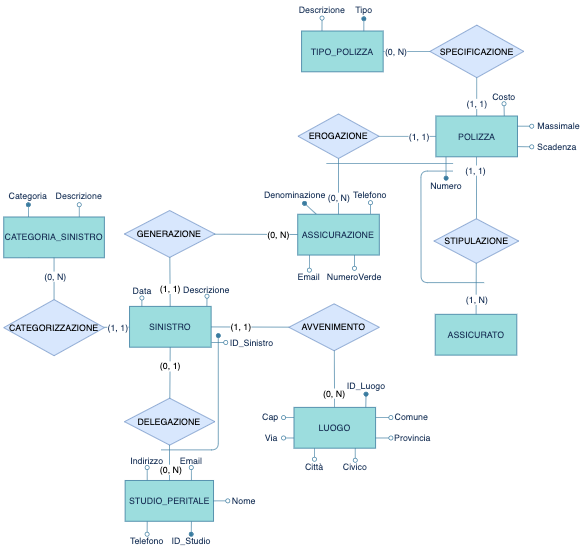
\includegraphics[width=\textwidth]{img/Assicurazione.png}
    \end{center}
\end{figure}
\clearpage

Dal dominio identificato in seguito all’intervista si può notare che sono presenti tre entità rappresentanti persone: \textbf{Perito}, \textbf{Supervisore} e \textbf{Assicurato}. Queste entità quindi sono generalizzate da \textbf{Persona} che raccoglie gli attributi in comune.
Nello specifico, per quanto riguarda l’assicurato, lo abbiamo messo in relazione con \textbf{Sinistro} per tenere traccia della parte coinvolta.
Ogni perito e ogni supervisore, potranno far parte solo di uno studio, mentre quest'ultimo potrà assumere diversi periti e supervisori.
Ogni supervisore potrà assegnare uno o più incarichi ad un perito, ma non necessariamente.
\\
\\
\\
\begin{figure}[ht]
    \begin{center}
        \centering
        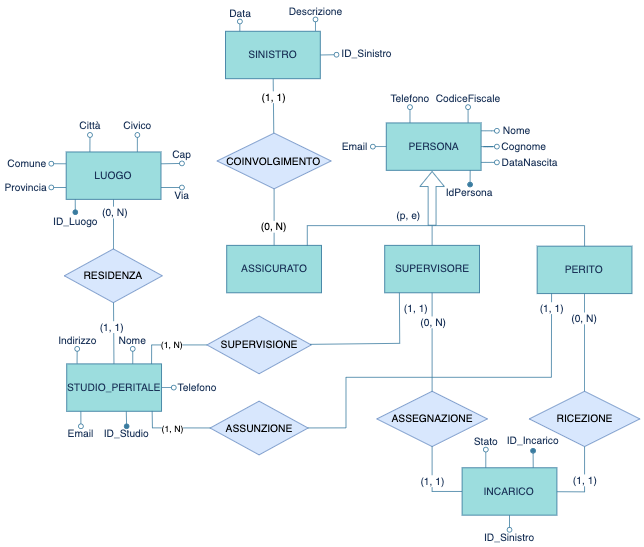
\includegraphics[width=\textwidth]{img/StudioPeritale.png}
    \end{center}
\end{figure}
\clearpage

Un perito, in un determinato momento, può non svolgere alcun \textbf{Incarico} ma può anche svolgerne molteplici, invece un incarico può essere svolto esclusivamente da un perito.
\\
Al momento della creazione di un incarico la video-perizia ovviamente non è ancora stata svolta, anche se ne deve essere presente almeno una al momento della chiusura dello stesso (per il corretto svolgimento delle attività peritali).
\\
La \textbf{Video\_perizia} può essere eseguita solo in presenza di un incarico, e quindi è identificata da un numero incrementale combinato al codice dell’incarico corrispondente.
\\
Durante la videochiamata possono essere acquisiti dei \textbf{Media} di tipo foto o video, ma non è sempre necessario. Questi ultimi, insieme ai documenti richiesti dal perito durante la video-perizia, sono stati generalizzati in File, dato che entrambi hanno una dimensione, un nome, un’estensione e una directory di appartenenza.
\\
Anche i \textbf{Documenti} possono essere di vari tipi (es: carta d’identità, verbale di sopralluogo, )
\\
I media in particolare dovranno contenere i metadati relativi alla posizione dell’assicurato durante la video-perizia.
\\
\begin{figure}[ht]
    \begin{center}
        \centering
        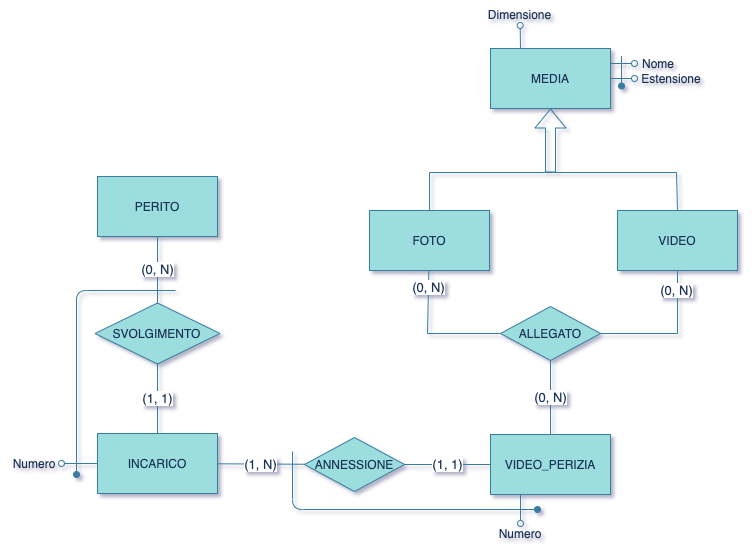
\includegraphics[width=\textwidth]{img/VideoPerizia.png}
    \end{center}
\end{figure}
\clearpage

\section{Schema concettuale finale}

\begin{figure}[ht]
    \begin{center}
        \centering
        \hspace*{-0.95in}
        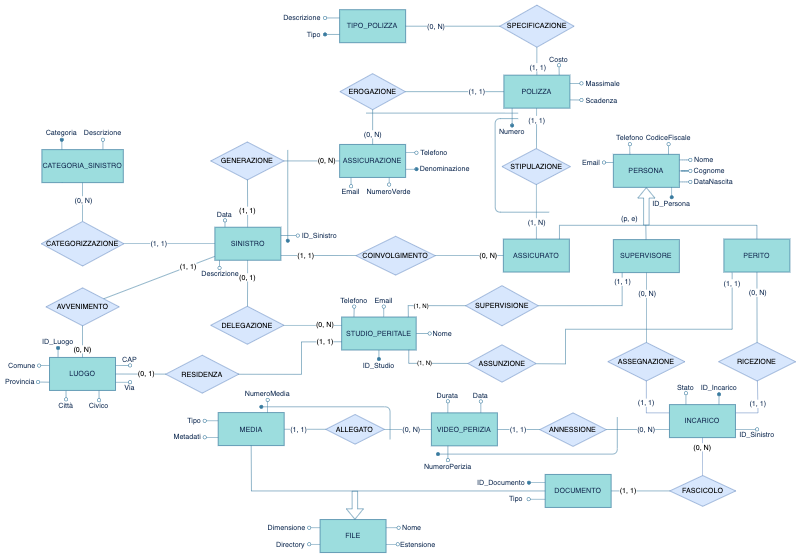
\includegraphics[scale=.64]{img/ER_Completo.png}
    \end{center}
\end{figure}
\chapter{Progettazione Logica}
\section{Stima del volume dei dati}

\mbox{}\\
\def\arraystretch{2}% 
\begin{tabularx}{\textwidth}{ p{6cm} | >{\centering\arraybackslash}p{2cm} | >{\centering\arraybackslash}X }
    \textbf{Concetto} & \textbf{Costrutto} & \textbf{Volume} \\
\hline
ASSICURAZIONE & E & 30\\ \hline
EROGAZIONE & A & 2.000.000\\ \hline
POLIZZA & E & 2.000.000\\ \hline
SPECIFICAZIONE & A & 2.000.000\\ \hline
TIPO\_POLIZZA & E & 15\\ \hline
STIPULAZIONE & A & 2.000.000\\ \hline
ASSICURATO & E & 1.000.000\\ \hline
LUOGO & E & 103.000\\ \hline
AVVENIMENTO & A & 150.000\\ \hline
RESIDENZA & A & 3.000\\ \hline
COINVOLGIMENTO & A & 150.000\\
\end{tabularx}

\noindent
\def\arraystretch{2}% 
\begin{tabularx}{\textwidth}{ p{6cm} | >{\centering\arraybackslash}p{2cm} | >{\centering\arraybackslash}X }
GENERAZIONE & A & 150.000\\ \hline
SINISTRO & E & 150.000\\ \hline
CATEGORIZZAZIONE & A & 150.000\\ \hline
CATEGORIA\_SINISTRO & E & 20\\ \hline
DELEGAZIONE & A & 150.000 \\ \hline
STUDIO\_PERITALE & E & 1.000\\ \hline
SUPERVISORE & E & 1.000\\ \hline
SUPERVISIONE & A & 1.000\\ \hline
PERITO & E & 7.000\\ \hline
ASSUNZIONE & A & 7.000\\ \hline
ASSEGNAZIONE & E & 150.000\\ \hline
RICEZIONE & A & 150.000\\ \hline
INCARICO & E & 150.000\\ \hline
FASCICOLO & A & 225.000\\ \hline
DOCUMENTO & E & 225.000\\ \hline
ANNESSIONE & A & 200.000\\ \hline
VIDEO\_PERIZIA & E & 200.000\\ \hline
ALLEGATO & A & 180.000\\ \hline
MEDIA & E & 180.000\\
\end{tabularx}

\clearpage
\section{Descrizione delle operazioni principali e stima della loro frequenza}

\def\arraystretch{2}% 
\begin{tabularx}{\textwidth}{ >{\centering\arraybackslash}p{2cm} | X |  >{\centering\arraybackslash}p{3cm} }
    \textbf{Codice} & \textbf{Operazione} & \textbf{Frequenza}\\
\hline
1 & Inserire un assicurato & 300 al giorno\\ \hline
2 & Visualizzare tutte le polizze di un assicurato & 50 al giorno\\ \hline
3 & Stipulazione di una nuova polizza tra assicurato e assicurazione & 1.000 al giorno\\ \hline
4 & Registrare un nuovo studio peritale & 5 al mese\\ \hline
5 & Rimuovere uno studio peritale & 5 al mese\\ \hline
6 & Generare un sinistro e delegarlo a uno studio peritale & 400 al giorno\\ \hline
7 & Assumere un supervisore in uno studio & 75 all'anno\\ \hline
8 & Licenziare il perito di uno studio & 150 all'anno\\ \hline
9 & Il supervisore crea un nuovo incarico e lo assegna a un perito & 400 al giorno\\ \hline
10 & Leggere tutti gli incarichi aperti in un determinato studio & 3.000 al giorno\\ \hline
11 & Visualizzare quale assicurato ha svolto una determinata video-perizia & 5.000 al giorno\\ 

\end{tabularx}

\noindent
\def\arraystretch{2}% 
\begin{tabularx}{\textwidth}{ >{\centering\arraybackslash}p{2cm} | X |  >{\centering\arraybackslash}p{3cm} }
12 & Aggiungere un documento ad un incarico & 600 al giorno\\ \hline
13 & Inserire una video-perizia per un incarico & 500 al giorno\\ \hline
14 & Visualizzare il proprietario (assicurato) di un documento & 5.000 al giorno\\ \hline
15 & Visualizzare in media quanto durano le video-perizie di un determinato studio peritale & 2.000 al giorno\\ \hline
16 & Visualizzare a quale sinistro è associato un determinato incarico & 5.000 al giorno
\end{tabularx}
\\
\\
\section{Schemi di navigazione e tabelle degli accessi}
In questa sezione verranno descritte le operazioni che non usufruiscono di ridondanze, per quelle con esse vedere il capitolo successivo.


\subsection{1 - Inserire un assicurato}
Inserire un assicurato implica che abbia stipulato un contratto con un assicurazione.
\\
\\
\def\arraystretch{2}% 
\begin{tabularx}{\textwidth}{ >{\centering\arraybackslash}p{3cm} | >{\centering\arraybackslash}X | >{\centering\arraybackslash}X |  >{\centering\arraybackslash}X }
    \textbf{Concetto} & \textbf{Costrutto} & \textbf{Accessi} & \textbf{Tipo} \\
\hline
Assicurato & E & 1 & S \\
Stipulazione & A & 1 & S \\
Polizza & E & 1 & S \\
Erogazione & A & 1 & S \\
\end{tabularx}
\begin{center}
\textbf{Totale : 4S * 300 al giorno = 2.400 al giorno}
\end{center}

\clearpage
\subsection{2 - Visualizzare tutte le polizze di un assicurato}
In media ogni assicurato avrà due polizze.
\\
\\
\def\arraystretch{2}% 
\begin{tabularx}{\textwidth}{ >{\centering\arraybackslash}p{3cm} | >{\centering\arraybackslash}X | >{\centering\arraybackslash}X |  >{\centering\arraybackslash}X }
    \textbf{Concetto} & \textbf{Costrutto} & \textbf{Accessi} & \textbf{Tipo} \\
\hline
Assicurato & E & 1 & L \\
Stipulazione & A & 2 & L \\
Polizza & E & 2 & L \\
\end{tabularx}
\begin{center}
\textbf{Totale : 5L * 50 al giorno = 250 al giorno}
\end{center}

\subsection{3 - Stipulazione di una nuova polizza tra assicurato e assicurazione}

\def\arraystretch{2}% 
\begin{tabularx}{\textwidth}{ >{\centering\arraybackslash}p{3cm} | >{\centering\arraybackslash}X | >{\centering\arraybackslash}X |  >{\centering\arraybackslash}X }
    \textbf{Concetto} & \textbf{Costrutto} & \textbf{Accessi} & \textbf{Tipo} \\
    \hline
    Stipulazione & A & 1 & S \\
    Polizza & E & 1 & S \\
    Erogazione & A & 1 & S \\
\end{tabularx}
\begin{center}
\textbf{Totale : 3S * 1.000 al giorno = 6.000 al giorno}
\end{center}
\clearpage
\subsection{4 - Registrare un nuovo studio peritale}
Inserire uno studio peritale ci vincola ad aggiungere anche almeno un dipendente e un supervisore, altrimenti lo studio non potrebbe assegnare lavori e svolgere incarichi, ciò vuol dire che si dovrà accedere in scrittura anche in Perito, Supervisore, e relative associazioni.
\\
\\
\def\arraystretch{2}% 
\begin{tabularx}{\textwidth}{ >{\centering\arraybackslash}p{3cm} | >{\centering\arraybackslash}X | >{\centering\arraybackslash}X |  >{\centering\arraybackslash}X }
    \textbf{Concetto} & \textbf{Costrutto} & \textbf{Accessi} & \textbf{Tipo} \\
    \hline
    Studio Peritale & E & 1 & S \\
    Supervisore & E & 1 & S \\
    Supervisione & A & 1 & S \\
    Assunzione & A & 1 & S \\
    Perito & E & 1 & S \\
\end{tabularx}
\begin{center}
\textbf{Totale : 5S * 5 al mese = 50 al mese}
\end{center}

\clearpage
\subsection{5 - Rimuovere uno studio peritale}
Rimuovere uno studio peritale implica che non si deve tenere più traccia dei dipendenti e degli incarichi dello studio, inoltre, deve essere eliminata la delegazione del sinistro, in modo tale che possa essere ri-delegato a un altro studio.
\\
Uno studio peritale in media ha 150 sinistri e incarichi, 7 periti e 1 supervisore.
\\
\\
\def\arraystretch{2}% 
\begin{tabularx}{\textwidth}{ >{\centering\arraybackslash}p{3cm} | >{\centering\arraybackslash}X | >{\centering\arraybackslash}X |  >{\centering\arraybackslash}X }
    \textbf{Concetto} & \textbf{Costrutto} & \textbf{Accessi} & \textbf{Tipo} \\
    \hline
    Studio Peritale & E & 1 & S \\
    Supervisore & E & 1 & S \\
    Supervisione & A & 1 & S \\
    Assunzione & A & 7 & S \\
    Perito & E & 7 & S \\
    Delegazione & A & 150 & S \\
    Assegnazione & A & 150 & S \\
    Incarico & E & 150 & S \\
    Ricezione & A & 150 & S \\
\end{tabularx}
\begin{center}
\textbf{Totale : 617S * 5 al mese = 6.170 al mese}
\end{center}
\clearpage

\subsection{6 - Generare un sinistro e delegarlo a uno studio peritale}
Quando si genera un sinistro si deve per forza specificare anche la categoria. Per quanto riguarda il luogo dell'avvenimento, non c'è alcun vincolo che mi impone di inserirne uno nuovo ogni volta, perchè il luogo in questione potrebbe essere già presente, tuttavia nella pratica la possibilità che sia così è bassissima, quasi nulla, per questo considero sempre una scrittura in Luogo.
\\
\\
\def\arraystretch{2}% 
\begin{tabularx}{\textwidth}{ >{\centering\arraybackslash}p{3cm} | >{\centering\arraybackslash}X | >{\centering\arraybackslash}X |  >{\centering\arraybackslash}X }
    \textbf{Concetto} & \textbf{Costrutto} & \textbf{Accessi} & \textbf{Tipo} \\
    \hline
    Generazione & A & 1 & S \\
    Sinistro & E & 1 & S \\
    Categorizzazione & A & 1 & S \\
    Delegazione & A & 1 & S \\
    Luogo & E & 1 & S \\
    Avvenimento & A & 1 & S \\
\end{tabularx}
\begin{center}
\textbf{Totale : 6S * 400 al giorno = 4.800 al giorno}
\end{center}

\subsection{7 - Assumere un supervisore in uno studio}
Quando si assume un supervisore (come quando si assume un perito) non c'è nessun vincolo da tenere in considerazione (a parte associarlo allo studio) quindi l'inserimento è immediato.
\\
\\
\def\arraystretch{2}% 
\begin{tabularx}{\textwidth}{ >{\centering\arraybackslash}p{3cm} | >{\centering\arraybackslash}X | >{\centering\arraybackslash}X |  >{\centering\arraybackslash}X }
    \textbf{Concetto} & \textbf{Costrutto} & \textbf{Accessi} & \textbf{Tipo} \\
    \hline
    Supervisore & E & 1 & S \\
    Supervisione & A & 1 & S \\
\end{tabularx}
\begin{center}
\textbf{Totale : 2S * 75 all'anno = 300 all'anno}
\end{center}

\clearpage
\subsection{8 - Licenziare il perito di uno studio}
Quando si licenzia un perito, il riferimento del perito in Incarico viene aggiornato automaticamente nel DB. 
\\
\\
\def\arraystretch{2}% 
\begin{tabularx}{\textwidth}{ >{\centering\arraybackslash}p{3cm} | >{\centering\arraybackslash}X | >{\centering\arraybackslash}X |  >{\centering\arraybackslash}X }
    \textbf{Concetto} & \textbf{Costrutto} & \textbf{Accessi} & \textbf{Tipo} \\
    \hline
    Perito & E & 1 & S \\
    Ricezione & A & 1 & S \\
    Incarico & E & 1 & S \\
\end{tabularx}
\begin{center}
\textbf{Totale : 2S * 150 all'anno = 600 all'anno}
\end{center}

\subsection{9 - Il supervisore crea un nuovo incarico e lo assegna a un perito}

\def\arraystretch{2}% 
\begin{tabularx}{\textwidth}{ >{\centering\arraybackslash}p{3cm} | >{\centering\arraybackslash}X | >{\centering\arraybackslash}X |  >{\centering\arraybackslash}X }
    \textbf{Concetto} & \textbf{Costrutto} & \textbf{Accessi} & \textbf{Tipo} \\
    \hline
    Ricezione & A & 1 & S \\
    Svolgimento & A & 1 & S \\
    Incarico & E & 1 & S \\
\end{tabularx}
\begin{center}
\textbf{Totale : 3S * 400 al giorno = 2.400 al giorno}
\end{center}

\clearpage

\subsection{10 - Leggere tutti gli incarichi aperti in un determinato studio}
Considerando che in media ogni studio peritale si occupa di 150 incarichi, e gli stati possono essere 2 (Aperto e Chiuso), avremo sempre in media 75 letture.
\\
\\
\def\arraystretch{2}% 
\begin{tabularx}{\textwidth}{ >{\centering\arraybackslash}p{3cm} | >{\centering\arraybackslash}X | >{\centering\arraybackslash}X |  >{\centering\arraybackslash}X }
    \textbf{Concetto} & \textbf{Costrutto} & \textbf{Accessi} & \textbf{Tipo} \\
    \hline
    Studio Peritale & E & 1 & L \\
    Incarico & E & 75 & L \\
\end{tabularx}
\begin{center}
\textbf{Totale : 76L * 3.000 al giorno = 228.000 al giorno}
\end{center}


\subsection{12 - Aggiungere un documento ad un incarico}
Un incarico in media include un fascicolo di 1/2 documenti.
\\
\\
\def\arraystretch{2}% 
\begin{tabularx}{\textwidth}{ >{\centering\arraybackslash}p{3cm} | >{\centering\arraybackslash}X | >{\centering\arraybackslash}X |  >{\centering\arraybackslash}X }
    \textbf{Concetto} & \textbf{Costrutto} & \textbf{Accessi} & \textbf{Tipo} \\
    \hline
    Documento & E & 1,5 & S \\
    Fascicolo & A & 1,5 & S \\
\end{tabularx}
\begin{center}
\textbf{Totale : 3S * 600 al giorno = 3.600 al giorno}
\end{center}

\subsection{13 - Inserire una video-perizia per un incarico}

\def\arraystretch{2}% 
\begin{tabularx}{\textwidth}{ >{\centering\arraybackslash}p{3cm} | >{\centering\arraybackslash}X | >{\centering\arraybackslash}X |  >{\centering\arraybackslash}X }
    \textbf{Concetto} & \textbf{Costrutto} & \textbf{Accessi} & \textbf{Tipo} \\
    \hline
    Video-Perizia & E & 1 & S \\
    Annessione & A & 1 & S \\
\end{tabularx}
\begin{center}
\textbf{Totale : 2S * 500 al giorno = 2.000 al giorno}
\end{center}

\subsection{15 - Visualizzare in media quanto durano le video-perizie di un determinato studio peritale}
In media ogni studio peritale esegue 200 video-perizie, di conseguenza andranno lette tutte per poter accedere alla durata di ognuna e farne una media.
\\
\\
\def\arraystretch{2}% 
\begin{tabularx}{\textwidth}{ >{\centering\arraybackslash}p{3cm} | >{\centering\arraybackslash}X | >{\centering\arraybackslash}X |  >{\centering\arraybackslash}X }
    \textbf{Concetto} & \textbf{Costrutto} & \textbf{Accessi} & \textbf{Tipo} \\
    \hline
    Studio Peritale & E & 1 & L \\
    Video-Perizia & E & 200 & L \\
    Annessione & A & 200 & L \\
\end{tabularx}
\begin{center}
\textbf{Totale : 401L * 2.000 al giorno = 802.000 al giorno}
\end{center}

\subsection{16 - Visualizzare a quale sinistro è associato un determinato incarico}

\def\arraystretch{2}% 
\begin{tabularx}{\textwidth}{ >{\centering\arraybackslash}p{3cm} | >{\centering\arraybackslash}X | >{\centering\arraybackslash}X |  >{\centering\arraybackslash}X }
    \textbf{Concetto} & \textbf{Costrutto} & \textbf{Accessi} & \textbf{Tipo} \\
    \hline
    Incarico & E & 1 & L \\
\end{tabularx}
\begin{center}
\textbf{Totale : 1L * 5.000 al giorno = 5.000 al giorno}
\end{center}

\clearpage
\section{Raffinamento dello schema}

\subsection{Eliminazione delle gerarchie}
Per l’eliminazione della gerarchia Persona si è scelto di adottare l’approccio del collasso verso il basso, replicando così gli attributi in Assicurato, Supervisore e Perito.
Si è scelta questa strategia in quanto si ha la necessità di trattare nello specifico ogni tipo di persona dando rilievo al ruolo di ognuna, per esempio bisogna ben diversificare i ruoli di Supervisore e Perito.
Per la gerarchia File si è seguita la stessa tecnica, quindi abbiamo replicato gli attributi comuni nelle entità figlie, poiché entrambe hanno ruoli ben distinti all'interno del dominio.
\\
\subsection{Eliminazione degli attributi composti}
Nello schema E/R non è presente alcun attributo composto, l'unico che esisteva in fase di progettazione concettuale era Luogo, ma poi si è deciso di elevarlo direttamente ad entità perché era di rilevante importanza sia per Sinistro che per Studio Peritale.
Sarà poi necessario accertarsi, a livello applicativo che gli attributi dell'entità Luogo coesistano senza dare origine a incoerenze (Esempio: non potranno esistere luoghi con un cap non corrispondente a quello della città).
\\
\subsection{Scelta delle chiavi primarie}
Nello schema sono già state specificate le chiavi primarie di tutte le entità, per quanto riguarda le entità della gerarchia Persona invece, si sceglie di usare come chiave primaria un ID univoco invece del codice fiscale, per riuscire a gestire anche i casi di omocodia.

\clearpage
\subsection{Eliminazione degli identificatori esterni}
Dallo schema principale sono state eliminate le seguenti relazioni:
\begin{itemize}
    \item \textbf{Specificazione}, importando Tipo in Polizza
    \item \textbf{Stipulazione}, importando ID\_Assicurato in Polizza
    \item \textbf{Erogazione}, importando Denominazione in Polizza
    \item \textbf{Coinvolgimento}, importando ID\_Assicurato in Sinistro
    \item \textbf{Generazione}, importando Denominazione in Sinistro
    \item \textbf{Categorizzazione}, importando Appellativo in Sinistro
    \item \textbf{Avvenimento}, importando ID\_Luogo in Sinistro
    \item \textbf{Residenza}, importando ID\_Luogo in Studio Peritale
    \item \textbf{Delegazione}, importando ID\_Studio in Sinistro
    \item \textbf{Supervisione}, importando ID\_Studio in Supervisore
    \item \textbf{Assunzione}, importando ID\_Studio in Perito
    \item \textbf{Assegnazione}, importando ID\_Supervisore in Incarico
    \item \textbf{Ricezione}, importando ID\_Perito in Incarico
    \item \textbf{Fascicolo}, importando ID\_Incarico in Documento
    \item \textbf{Annessione}, importando ID\_Incarico in Video\_Perizia
    \item \textbf{Allegato}, importando NumeroPerizia ID\_Incarico in Media
\end{itemize}
\clearpage
\section{Analisi delle ridondanze}
Si è deciso di inserire ID\_Assicurato sia in Documento sia in Video\_Perizia perché sono molto frequenti le operazioni che associano i vari documenti e video-perizie alla parte coinvolta. Di seguito è mostrata la differenza tra i due casi, in termini di accessi, in entrambe le operazioni.
\\
\subsection{11 - Visualizzare quale assicurato ha svolto una determinata video-perizia}

\textbf{Senza ridondanza}
\\
\\
\def\arraystretch{2}% 
\begin{tabularx}{\textwidth}{ >{\centering\arraybackslash}p{3cm} | >{\centering\arraybackslash}X | >{\centering\arraybackslash}X |  >{\centering\arraybackslash}X }
    \textbf{Concetto} & \textbf{Costrutto} & \textbf{Accessi} & \textbf{Tipo} \\
    \hline
    Video-perizia & E & 1 & L \\
    Annessione & A & 1 & L \\
    Incarico & E & 1 & L \\
    Sinistro & E & 1 & L \\
    Coinvolgimento & A & 1 & L \\
    Assicurato & E & 1 & L \\
\end{tabularx}
\begin{center}
\textbf{Totale : 6L * 5.000 al giorno = 30.000 al giorno}
\end{center}

\textbf{Con ridondanza}
\\
\\
\def\arraystretch{2}% 
\begin{tabularx}{\textwidth}{ >{\centering\arraybackslash}p{3cm} | >{\centering\arraybackslash}X | >{\centering\arraybackslash}X |  >{\centering\arraybackslash}X }
    \textbf{Concetto} & \textbf{Costrutto} & \textbf{Accessi} & \textbf{Tipo} \\
    \hline
    Video-perizia & E & 1 & L \\
\end{tabularx}
\begin{center}
\textbf{Totale : 1L * 5.000 al giorno = 5.000 al giorno}
\end{center}

\clearpage

\subsection{14 - Visualizzare il proprietario (assicurato) di un documento}

\textbf{Senza ridondanza}
\\
\\
\def\arraystretch{2}% 
\begin{tabularx}{\textwidth}{ >{\centering\arraybackslash}p{3cm} | >{\centering\arraybackslash}X | >{\centering\arraybackslash}X |  >{\centering\arraybackslash}X }
    \textbf{Concetto} & \textbf{Costrutto} & \textbf{Accessi} & \textbf{Tipo} \\
    \hline
    Documento & E & 1 & L \\
    Fascicolo & A & 1 & L \\
    Incarico & E & 1 & L \\
    Sinistro & E & 1 & L \\
    Coinvolgimento & A & 1 & L \\
    Assicurato & E & 1 & L \\
\end{tabularx}
\begin{center}
\textbf{Totale : 6L * 5.000 al giorno = 30.000 al giorno}
\end{center}

\textbf{Con ridondanza}
\\
\\
\def\arraystretch{2}% 
\begin{tabularx}{\textwidth}{ >{\centering\arraybackslash}p{3cm} | >{\centering\arraybackslash}X | >{\centering\arraybackslash}X |  >{\centering\arraybackslash}X }
    \textbf{Concetto} & \textbf{Costrutto} & \textbf{Accessi} & \textbf{Tipo} \\
    \hline
   Documento & E & 1 & L \\
\end{tabularx}
\begin{center}
\textbf{Totale : 1L * 5.000 al giorno = 5.000 al giorno}
\end{center}

\clearpage

\section{Traduzione di entità e associazioni in relazioni}

\textbf{Assicurati}(\underline{ID\_Assicurato}, Nome, Cognome, DataNascita, CodiceFiscale, Telefono, Email)
\\
\\
\textbf{Polizze}(\underline{Numero}, \underline{Assicurato}, \underline{Assicurazione} Massimale, Costo, Scadenza, Tipo) \\
FK: Assicurato \texttt{REFERENCES} Assicurati \\
FK: Assicurazione \texttt{REFERENCES} Assicurazioni \\
FK: Tipo \texttt{REFERENCES} Tipi\_Polizze  \\
\\
\textbf{Tipi\_Polizze}(\underline{Tipo}, Descrizione)
\\
\\
\textbf{Assicurazioni}(\underline{Denominazione}, Email, Telefono, NumeroVerde) \\
\\
\textbf{Categorie\_Sinistri}(\underline{Appellativo}, Descrizione) \\
\\
\textbf{Sinistri}(\underline{ID\_Sinistro}, \underline{Assicurazione}, Descrizione, Data,  Categoria, Luogo, Assicurato, StudioPeritale) \\
FK: Assicurazione \texttt{REFERENCES} Assicurazioni \\
FK: Assicurato \texttt{REFERENCES} Assicurati \\
FK: Categoria \texttt{REFERENCES} Categorie\_Sinistri  \\
FK: Luogo \texttt{REFERENCES} Luoghi \\
FK: StudioPeritale \texttt{REFERENCES} Studi\_Peritali \\
\\
\textbf{Luoghi}(\underline{ID\_Luogo}, Via, NumeroCivico, Citta, Comune, Provincia, CAP) \\
\\
\textbf{Studi\_Peritali}(\underline{ID\_Studio},  Nome, Email, Telefono, Luogo) \\
FK: Luogo \texttt{REFERENCES} Luoghi \\
\\
\textbf{Supervisori}(\underline{ID\_Supervisore}, Nome, Cognome, DataNascita, CodiceFiscale, Telefono, Email) \\
FK: Studio \texttt{REFERENCES} Studi\_Peritali \\
\\
\textbf{Periti}(\underline{ID\_Perito}, Nome, Cognome, DataNascita, CodiceFiscale, Telefono, Email) \\
FK: Studio \texttt{REFERENCES} Studi\_Peritali \\
\clearpage
\noindent
\textbf{Incarichi}(\underline{ID\_Incarico}, ID\_Sinistro, Stato, Supervisore, Perito) \\
FK: Supervisore \texttt{REFERENCES} Supervisori \\
FK: Perito \texttt{REFERENCES} Periti \\
\\
\textbf{Documenti}(\underline{ID\_Documento}, Nome, Estensione, Dimensione, Directory, Tipo, ID\_Assicurato, Incarico) \\
FK: Incarico \texttt{REFERENCES} Incarichi \\
\\
\textbf{Video\_Perizie}(\underline{NumeroPerizia}, \underline{Incarico}, Durata) \\
FK: Incarico \texttt{REFERENCES} Incarichi \\
\\
\textbf{Media}(\underline{NumeroMedia}, \underline{Video\_Perizia}, \underline{Incarico}, Nome, Estensione, Dimensione, Directory, Tipo, Metadati) \\
FK: Incarico \texttt{REFERENCES} Incarichi \\
FK: Video\_Perizia \texttt{REFERENCES} Video\_Perizie \\

\clearpage
\section{Schema relazionale finale}

\begin{figure}[ht]
    \begin{center}
        \centering
        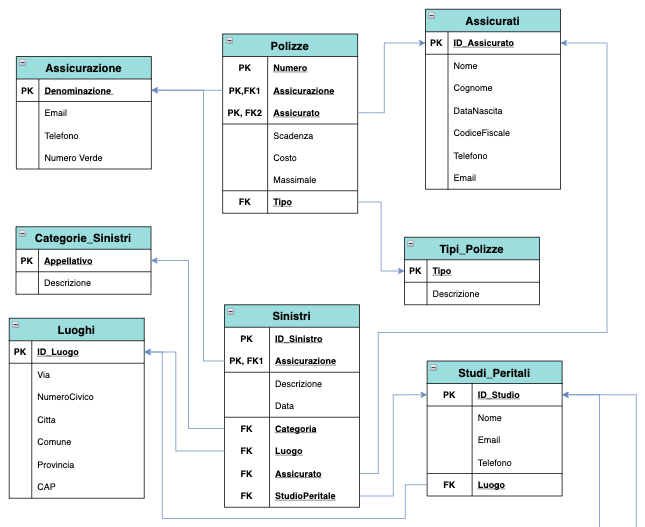
\includegraphics[width=\textwidth]{img/Relazionale1.png}
    \end{center}
\end{figure}

\clearpage
\begin{figure}[ht]
    \begin{center}
        \centering
        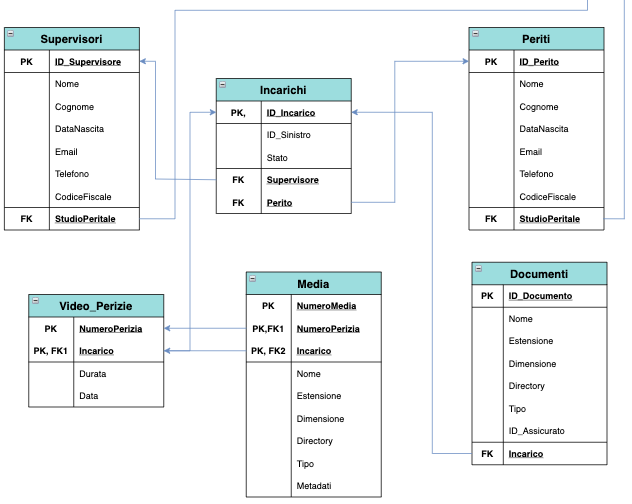
\includegraphics[width=\textwidth]{img/Relazionale2.png}
    \end{center}
\end{figure}

\clearpage
\section{Traduzione delle operazioni in query SQL}

Nelle query di inserimento, se viene omesso l'identificativo del record è perché la chiave primaria in quel caso è auto incrementale.

\definecolor{backcolour}{rgb}{0.96,0.96,0.96}
\definecolor{codegreen}{rgb}{0,0.6,0}
\definecolor{codegray}{rgb}{0.5,0.5,0.5}
\definecolor{codepurple}{rgb}{0.58,0,0.82}

\lstdefinestyle{mystyle}{
    backgroundcolor=\color{backcolour},   
    commentstyle=\color{codegreen},
    keywordstyle=\color{blue},
    numberstyle=\tiny\color{codegray},
    stringstyle=\color{codepurple},
    basicstyle=\ttfamily\footnotesize,
    breakatwhitespace=false,         
    breaklines=true,                 
    captionpos=b,                    
    keepspaces=true,                 
    numbers=left,                    
    numbersep=5pt,                  
    showspaces=false,                
    showstringspaces=false,
    showtabs=false,                  
    tabsize=2
}

\lstset{style=mystyle}
\begin{lstlisting}[language=SQL]
/* 
    Operazione 1 - Inserire un assicurato
*/
BEGIN TRANSACTION;
    DECLARE @Assicurato INT
    SET @Assicurato = (SELECT TOP 1 ID_Assicurato
                    FROM Assicurati
                    ORDER BY ID_Assicurato DESC) + 1;
    INSERT INTO Assicurati (Nome, Cognome, DataNascita, CodiceFiscale, Telefono, Email) 
    VALUES (?, ?, ?, ?, ?, ?);
    INSERT INTO Polizze (Tipo, Assicurato, Assicurazione, Massimale, Costo, Scadenza) 
    VALUES (?, @Assicurato, ?, ?, ?, ?);
COMMIT;

/*
    Operazione 2 - Visualizzare tutte le polizze di un assicurato
*/
SELECT *
FROM Polizze
WHERE Assicurato = ?;

/*
    Operazione 3 - Stipulazione di una nuova polizza tra assicurato e  assicurazione
*/
INSERT INTO Polizze (Tipo, Assicurato, Assicurazione, Massimale, Costo, Scadenza) 
VALUES (?, ?, ?, ?, ?, ?);

/*
    Operazione 4 - Registrare un nuovo studio peritale 
*/
BEGIN TRANSACTION;
    INSERT INTO Luoghi (Provincia, Via, NumeroCivico, CAP, Comune, Citta)
    VALUES (?, ?, ?, ?, ?, ?);
    INSERT INTO Studi_Peritali (Luogo, Nome, Telefono, Email) 
    VALUES (?, ?, ?, ?);
    INSERT INTO Supervisori (Nome, Cognome, DataNascita, CodiceFiscale, Telefono, Email) 
    VALUES (?, ?, ?, ?, ?, ?);
    INSERT INTO Periti (Nome, Cognome, DataNascita, CodiceFiscale, Telefono, Email) 
    VALUES (?, ?, ?, ?, ?, ?);
COMMIT;

/*
    Operazione 5 - Rimuovere uno studio peritale 
*/
DELETE FROM Studi_Peritali WHERE ?;

/*
    Operazione 6 - Generare un sinistro e delegarlo a uno studio peritale
*/
INSERT INTO Sinistri (ID_Sinistro, Assicurazione, Descrizione, Data, Categoria, Luogo, Studio_Peritale, Assicurato)
VALUES (?, ?, ?, ?, ?, ?, ?, ?)

/*
    Operazione 7 - Assumere un supervisore in uno studio
*/
INSERT INTO Supervisori (Nome, Cognome, DataNascita, CodiceFiscale, Telefono, Email) 
VALUES (?, ?, ?, ?, ?, ?);

/*
    Operazione 8 - Licenziare il perito di uno studio 
*/
DELETE FROM Perito
WHERE ?;

/*
    Operazione 9 - Il  supervisore  crea  un  nuovo  incarico  e  lo  assegna  a  un perito 
*/
INSERT INTO Incarichi (Perito, Supervisore, ID_Sinistro, Stato)
VALUES (?, ?, ?, ?);

/*
    Operazione 10 - Leggere tutti gli incarichi aperti in un determinato studio
*/
SELECT *
FROM Incarichi
WHERE Stato == 'Aperto' AND ID_Studio = ?;

/*
    Operazione 11 - Visualizzare quale assicurato ha svolto una determinata video-perizia 
*/
SELECT ID_Assicurato
FROM Video_Perizie
WHERE ?;

/*
    Operazione 12 - Aggiungere un documento ad un incarico 
*/
INSERT INTO Documenti (ID_Incarico, Incarico, Tipo)
VALUES (?, ?, ?);

/*
    Operazione 13 - Inserire una video-perizia per un incarico 
*/
INSERT INTO Video_Perizie (Incarico, Durata)
VALUES (?, ?);

/*
    Operazione 14 - Visualizzare il proprietario (assicurato) di un documento
*/
SELECT ID_Assicurato
FROM Documenti
WHERE ?;

/*
    Operazione 15 - Visualizzare in media quanto durano le video-perizie di un determinato studio peritale 
*/
SELECT AVG(Durata) AS DurataMedia
FROM Video_Perizie AS Perizie
INNER JOIN Incarichi 
ON Perizie.Incarico = Incarichi.ID_Incarico
INNER JOIN Supervisori
ON Incarichi.Supervisore = Supervisori.ID_Supervisore
INNER JOIN Studi_Peritali 
ON Supervisori.Studio = Studi_Peritali.ID_Studio
WHERE Studio = ?;

/*
    Operazione 16 - Qual e' la provincia nella quale avvengono piu' sinistri
*/
SELECT TOP 1 Provincia, COUNT(*) as TotaleIncarichi
FROM Sinistri 
INNER JOIN Luoghi
ON Sinistri.ID_Luogo = Luoghi.ID_Luogo
GROUP BY Provincia
ORDER BY TotaleIncarichi DESC;
\end{lstlisting}





\chapter{Progettazione dell'applicazione}

Per sviluppare l'applicazione si è scelto di usare SQL Server e il linguaggio C\#.
Abbiamo creato un'applicazione WPF per creare una semplice interfaccia grafica.
Inoltre si è utilizzato LINQ per eseguire le interrogazioni al database sfruttando le funzionalità della programmazione ad oggetti.
L'applicazione è divisa in sezioni, in seguito verranno mostrate le principali funzionalità.

\section{Visualizza}
Si possono visualizzare tutti i record di tutte le tabelle del database, senza alcuna condizione

\begin{figure}[ht]
    \begin{center}
        \centering
        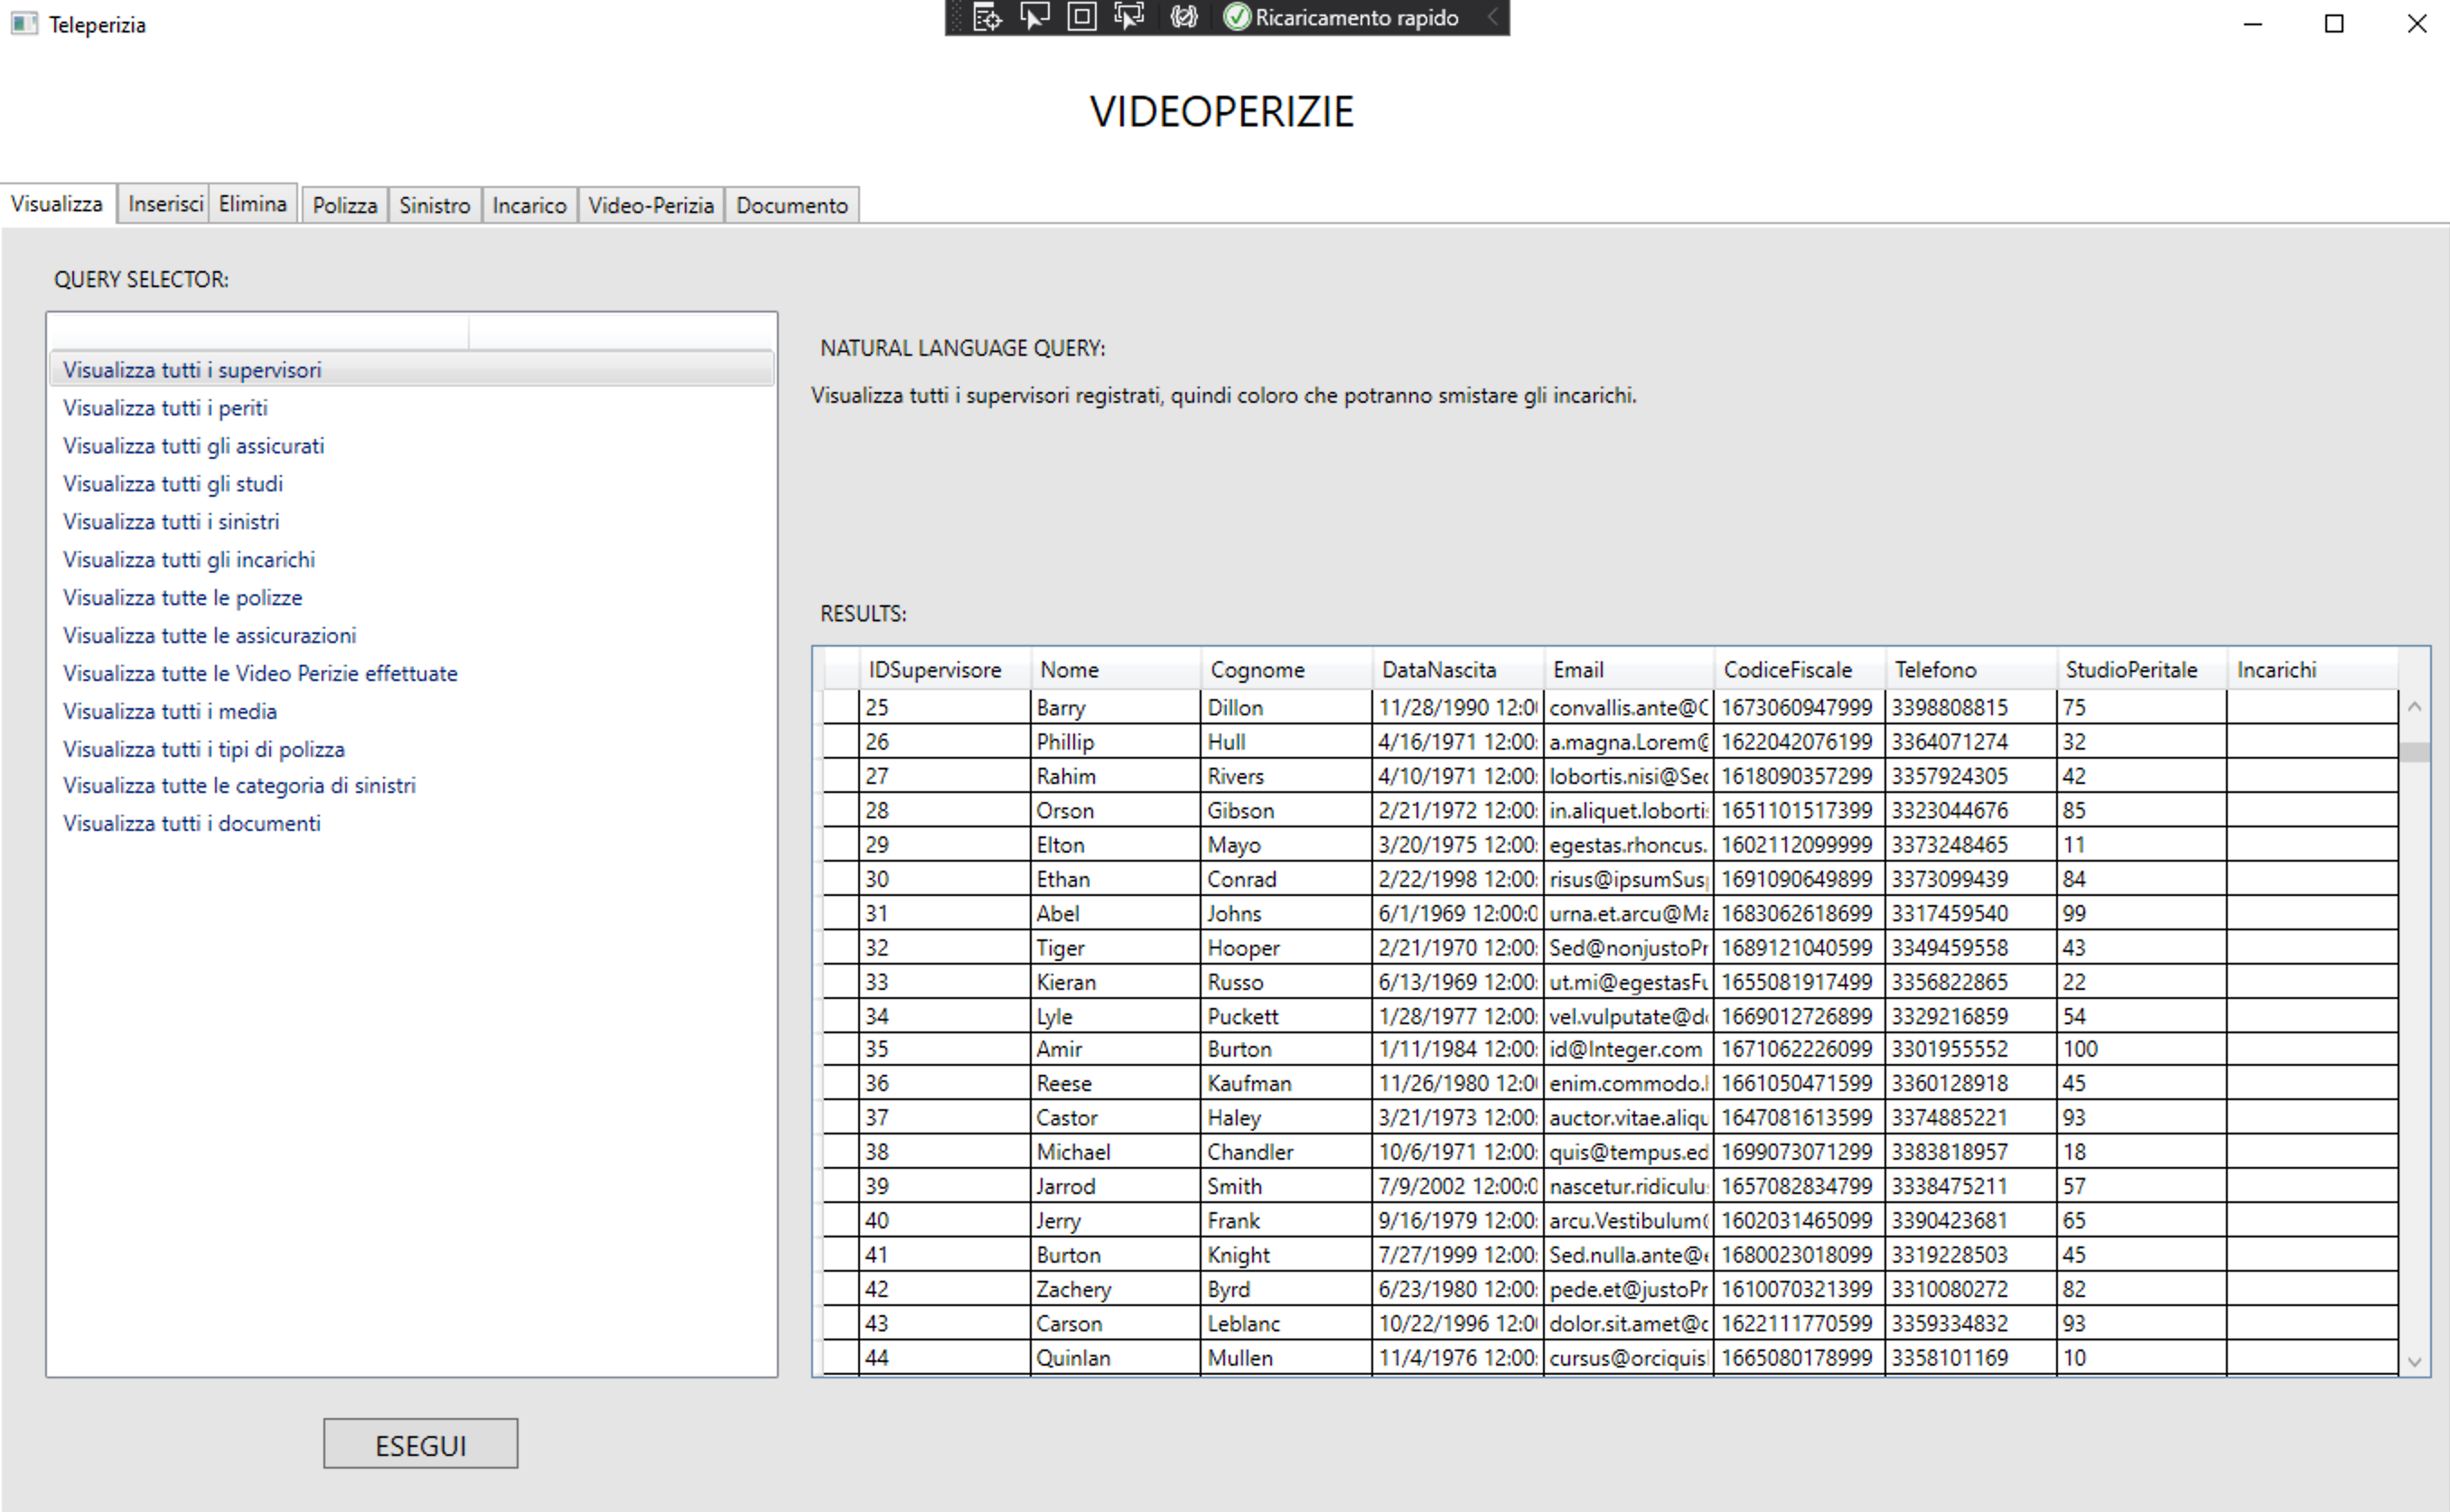
\includegraphics[scale=0.3]{img/Applicazione/Visualizza.png}
    \end{center}
\end{figure}
\clearpage

\section{Inserisci}
Si possono inserire vari tipi di record in quasi tutte le tabelle, rispettando sempre i vincoli impostati durante la creazione del database

\begin{figure}[ht]
    \begin{center}
        \centering
        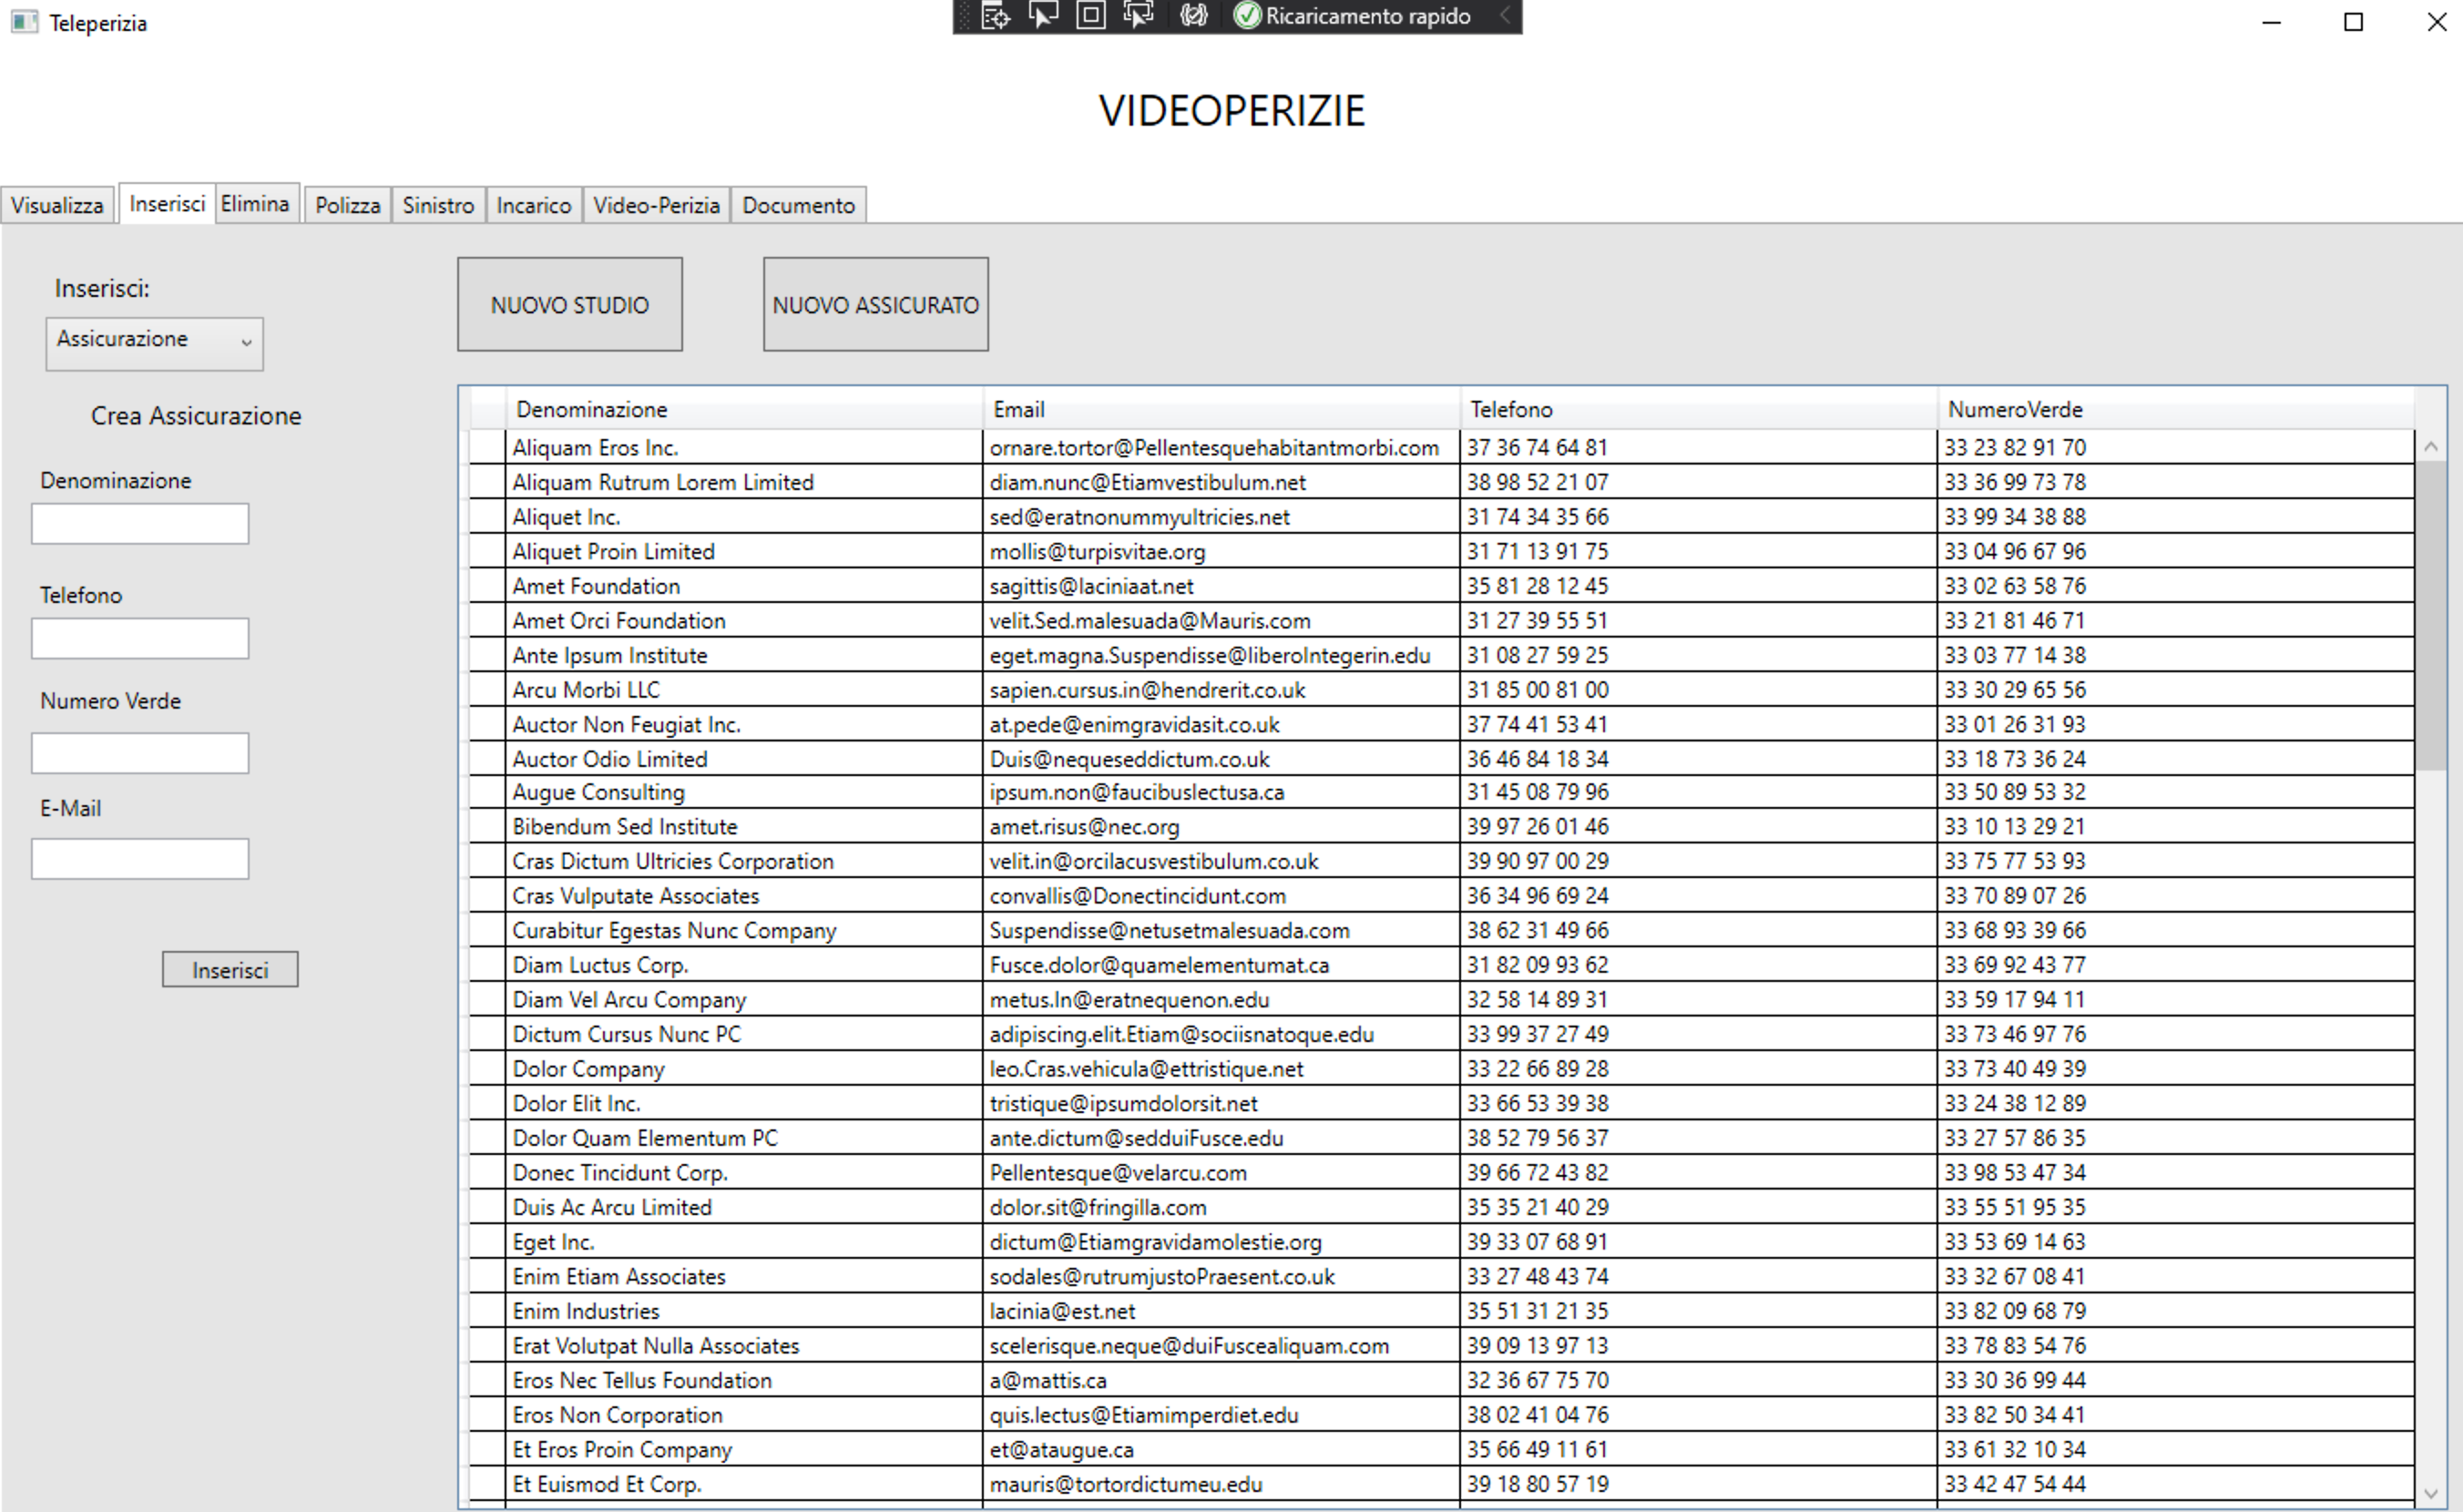
\includegraphics[width=\textwidth]{img/Applicazione/Inserisci1.png}
    \end{center}
\end{figure}
\clearpage
\begin{figure}[ht]
    \begin{center}
        \centering
        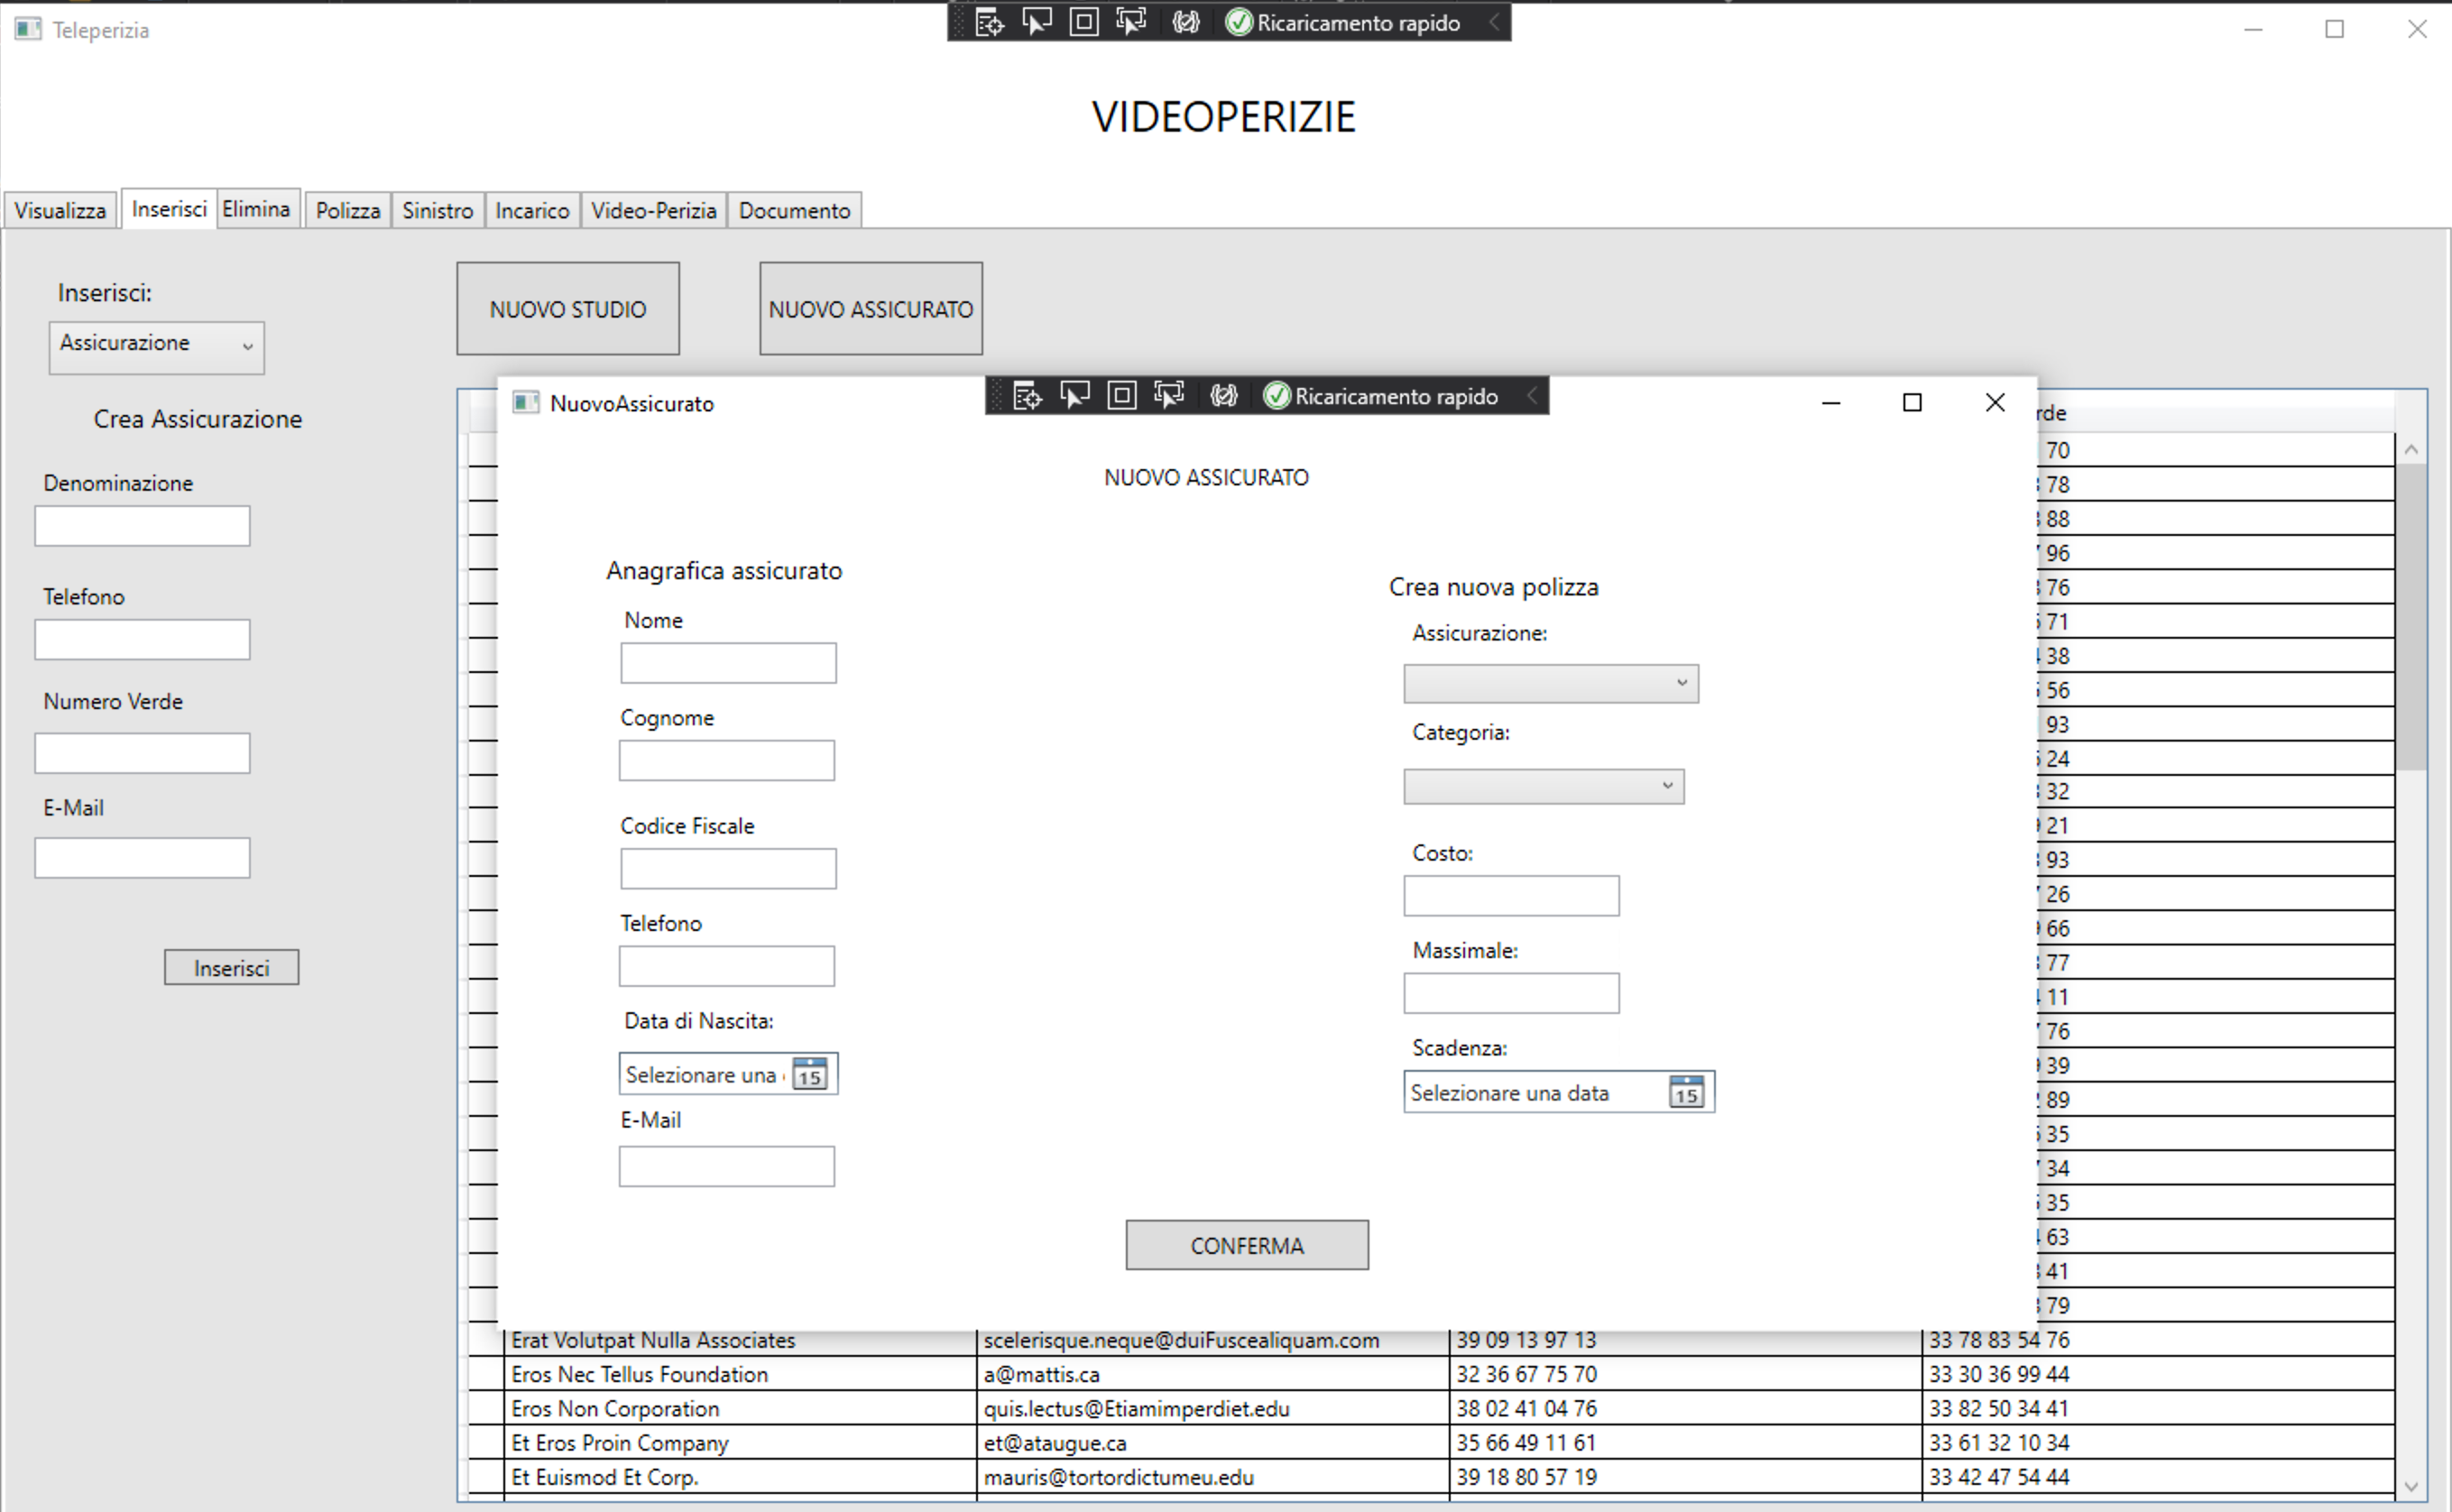
\includegraphics[width=\textwidth]{img/Applicazione/Inserisci2.png}
    \end{center}
\end{figure}
\clearpage
\begin{figure}[ht]
    \begin{center}
        \centering
        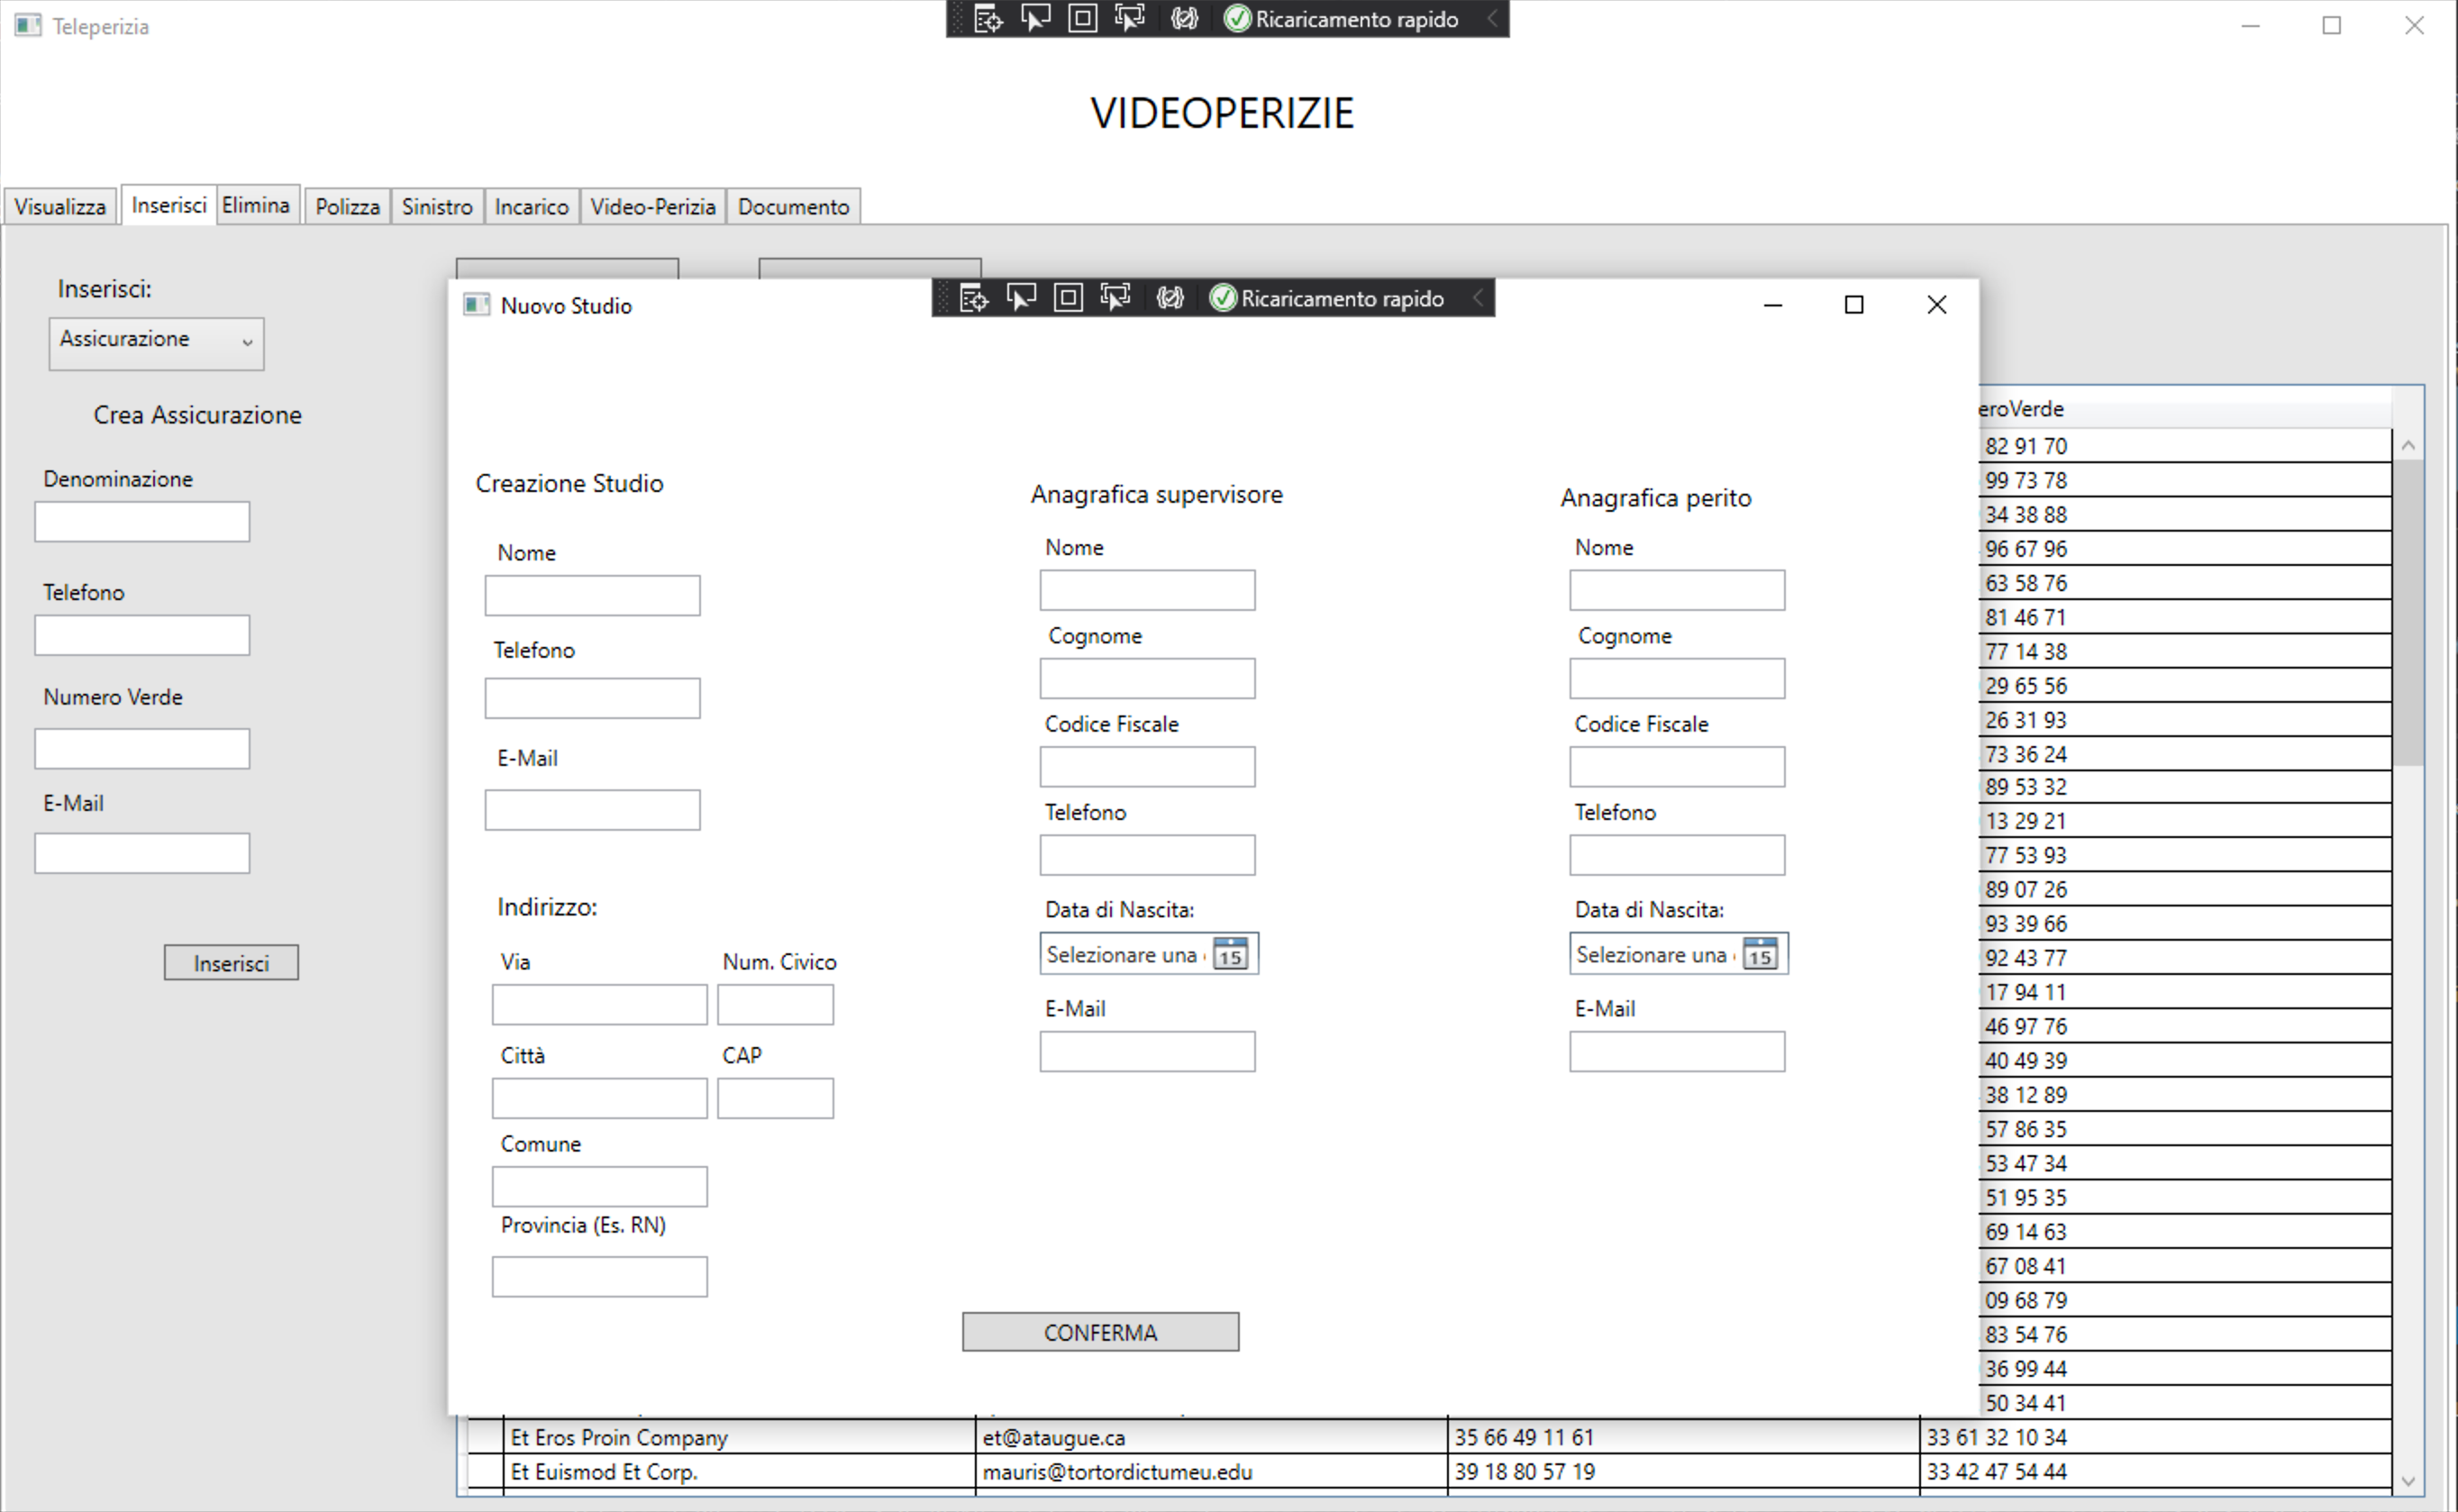
\includegraphics[width=\textwidth]{img/Applicazione/Inserisci3.png}
    \end{center}
\end{figure}
\clearpage
\section{Elimina}
Si possono eliminare i record dato in input la chiave primaria correttamente

\begin{figure}[ht]
    \begin{center}
        \centering
        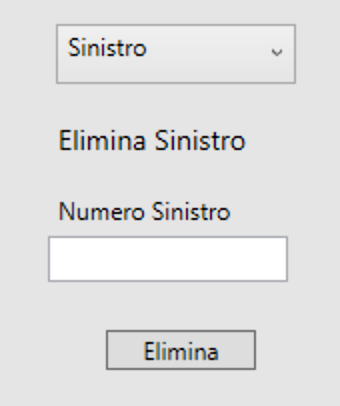
\includegraphics[scale=1]{img/Applicazione/Elimina.png}
    \end{center}
\end{figure}

\clearpage
\section{Polizza}
Si possono gestire le stipulazioni di nuove polizze tra assicurati e assicurazioni.

\begin{figure}[ht]
    \begin{center}
        \centering
        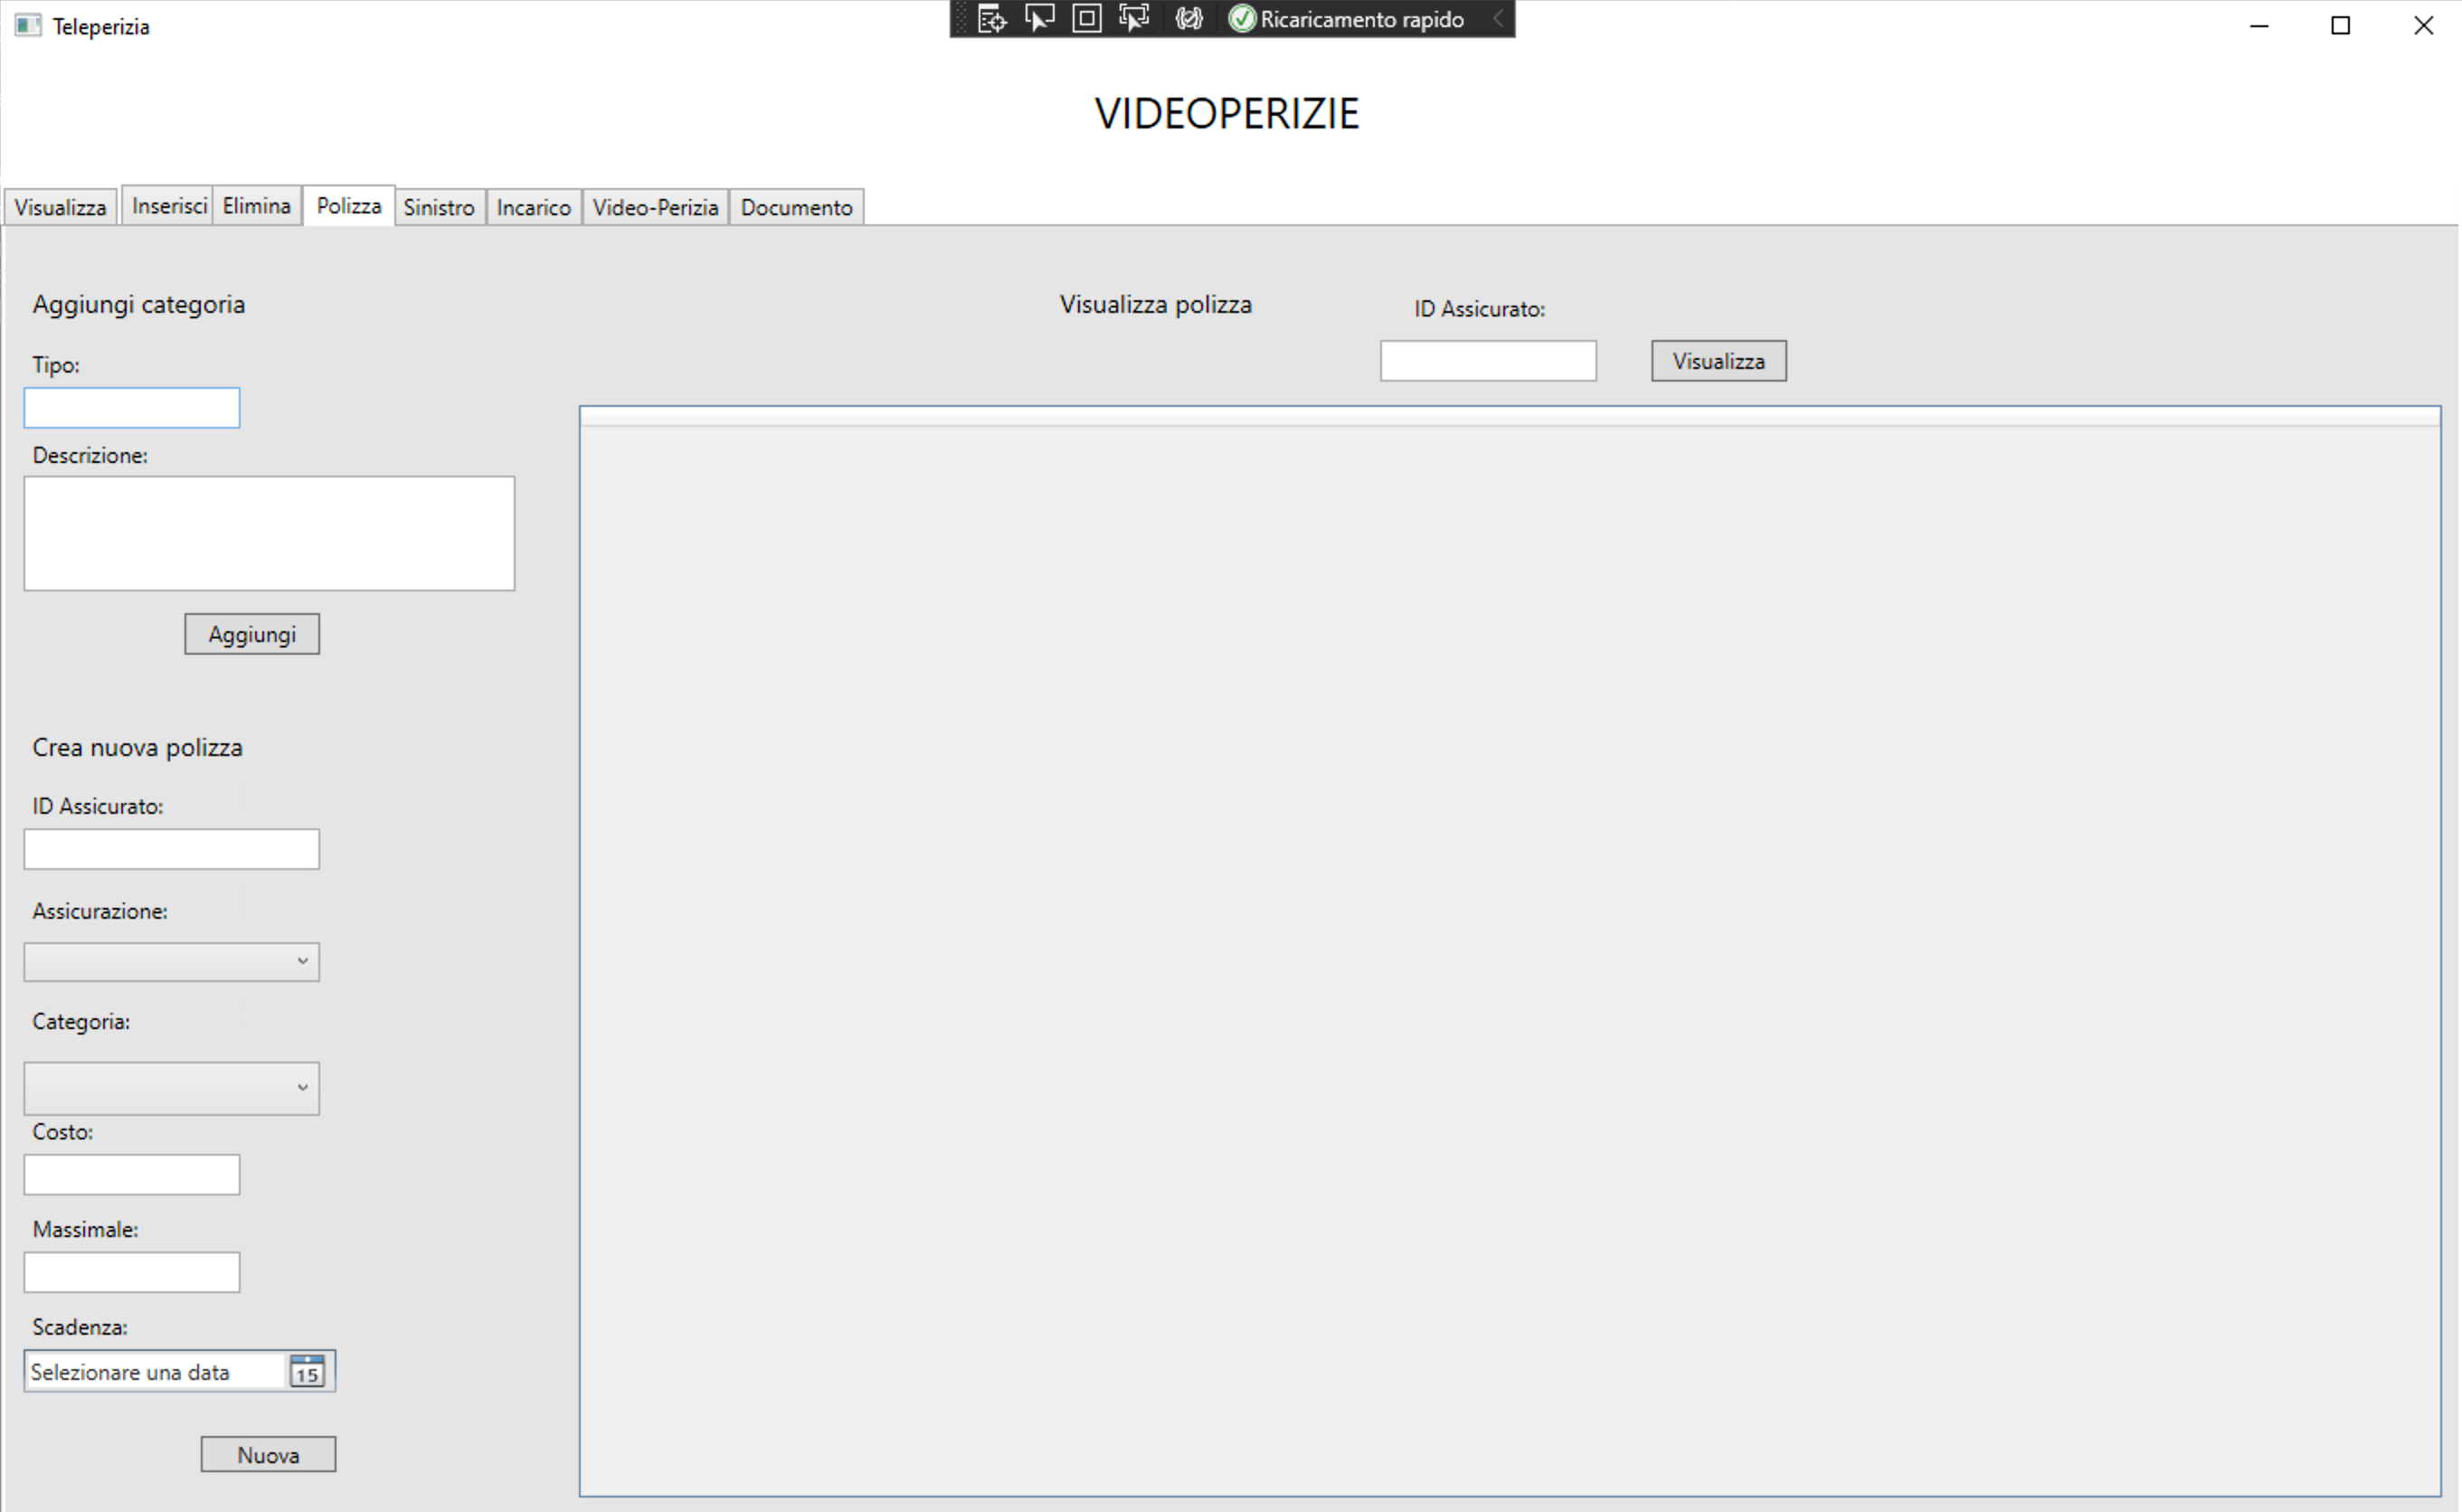
\includegraphics[width=\textwidth]{img/Applicazione/Polizza.png}
    \end{center}
\end{figure}
\clearpage
\section{Sinistro}
Si possono gestire i sinistri generati dalle assicurazioni, si può decidere di delegarli subito a uno studio peritale oppure farlo successivamente.

\begin{figure}[ht]
    \begin{center}
        \centering
        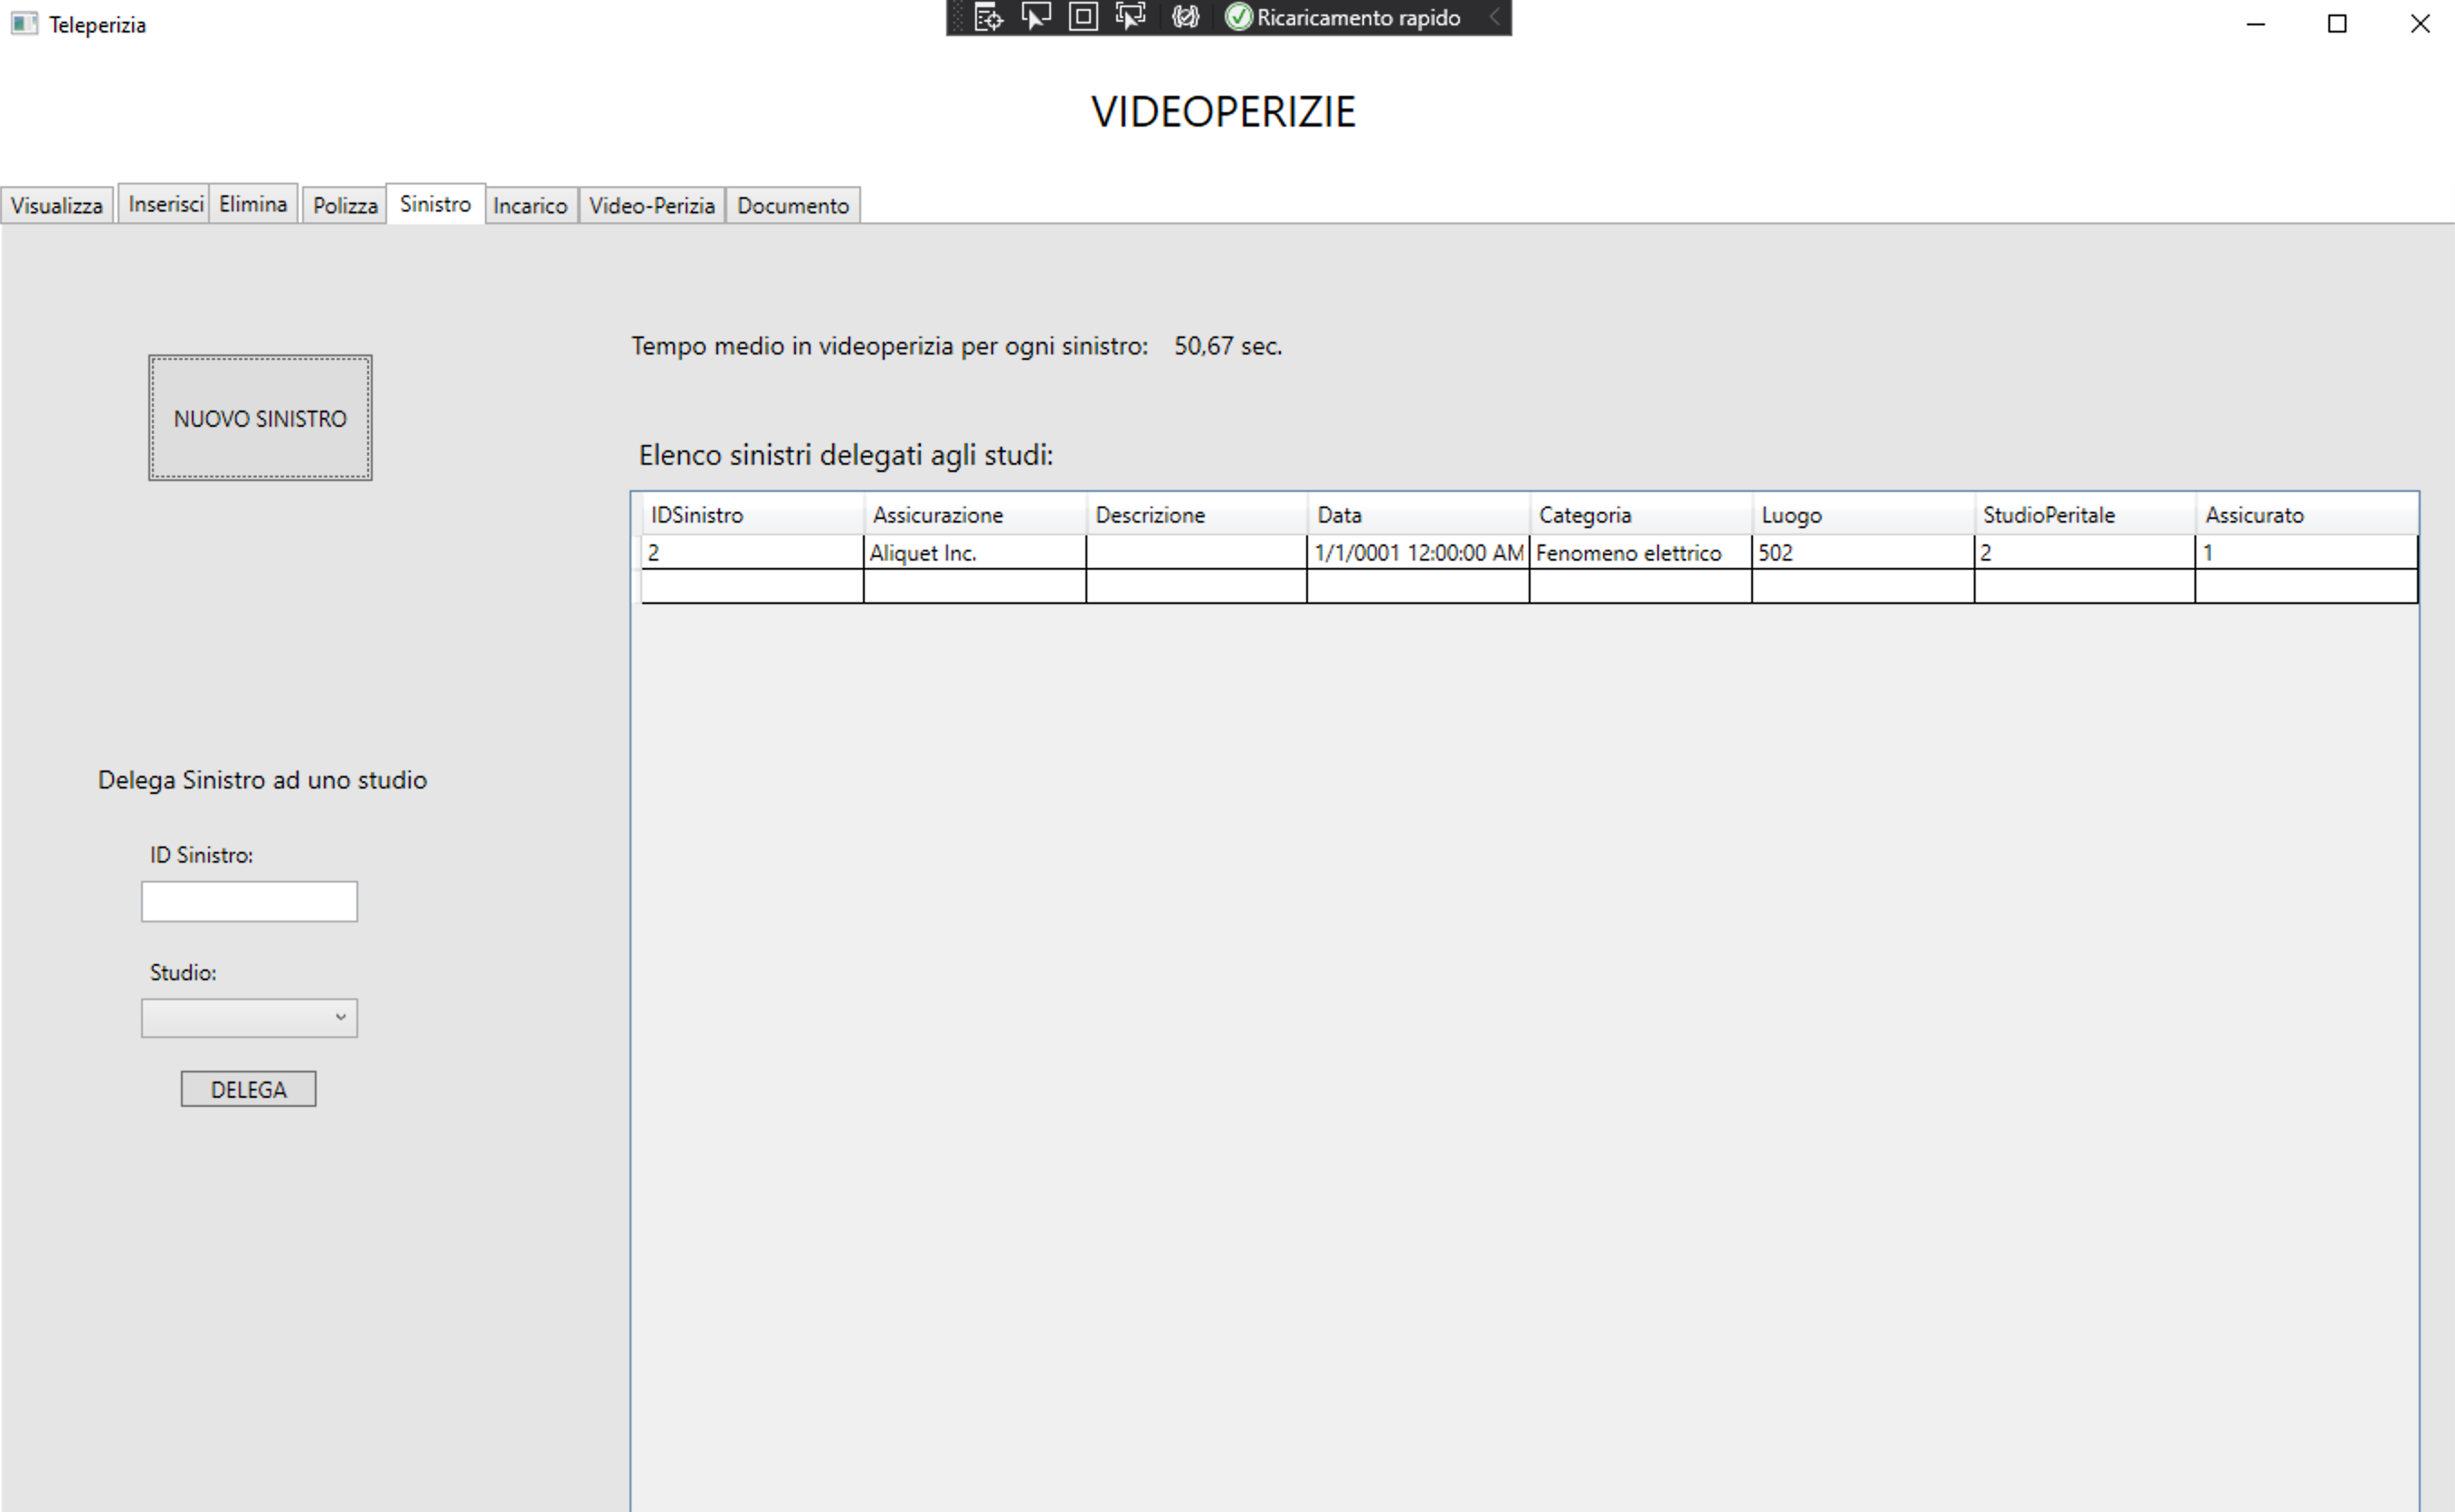
\includegraphics[width=\textwidth]{img/Applicazione/Sinistro1.png}
    \end{center}
\end{figure}

\clearpage

\begin{figure}[ht]
    \begin{center}
        \centering
        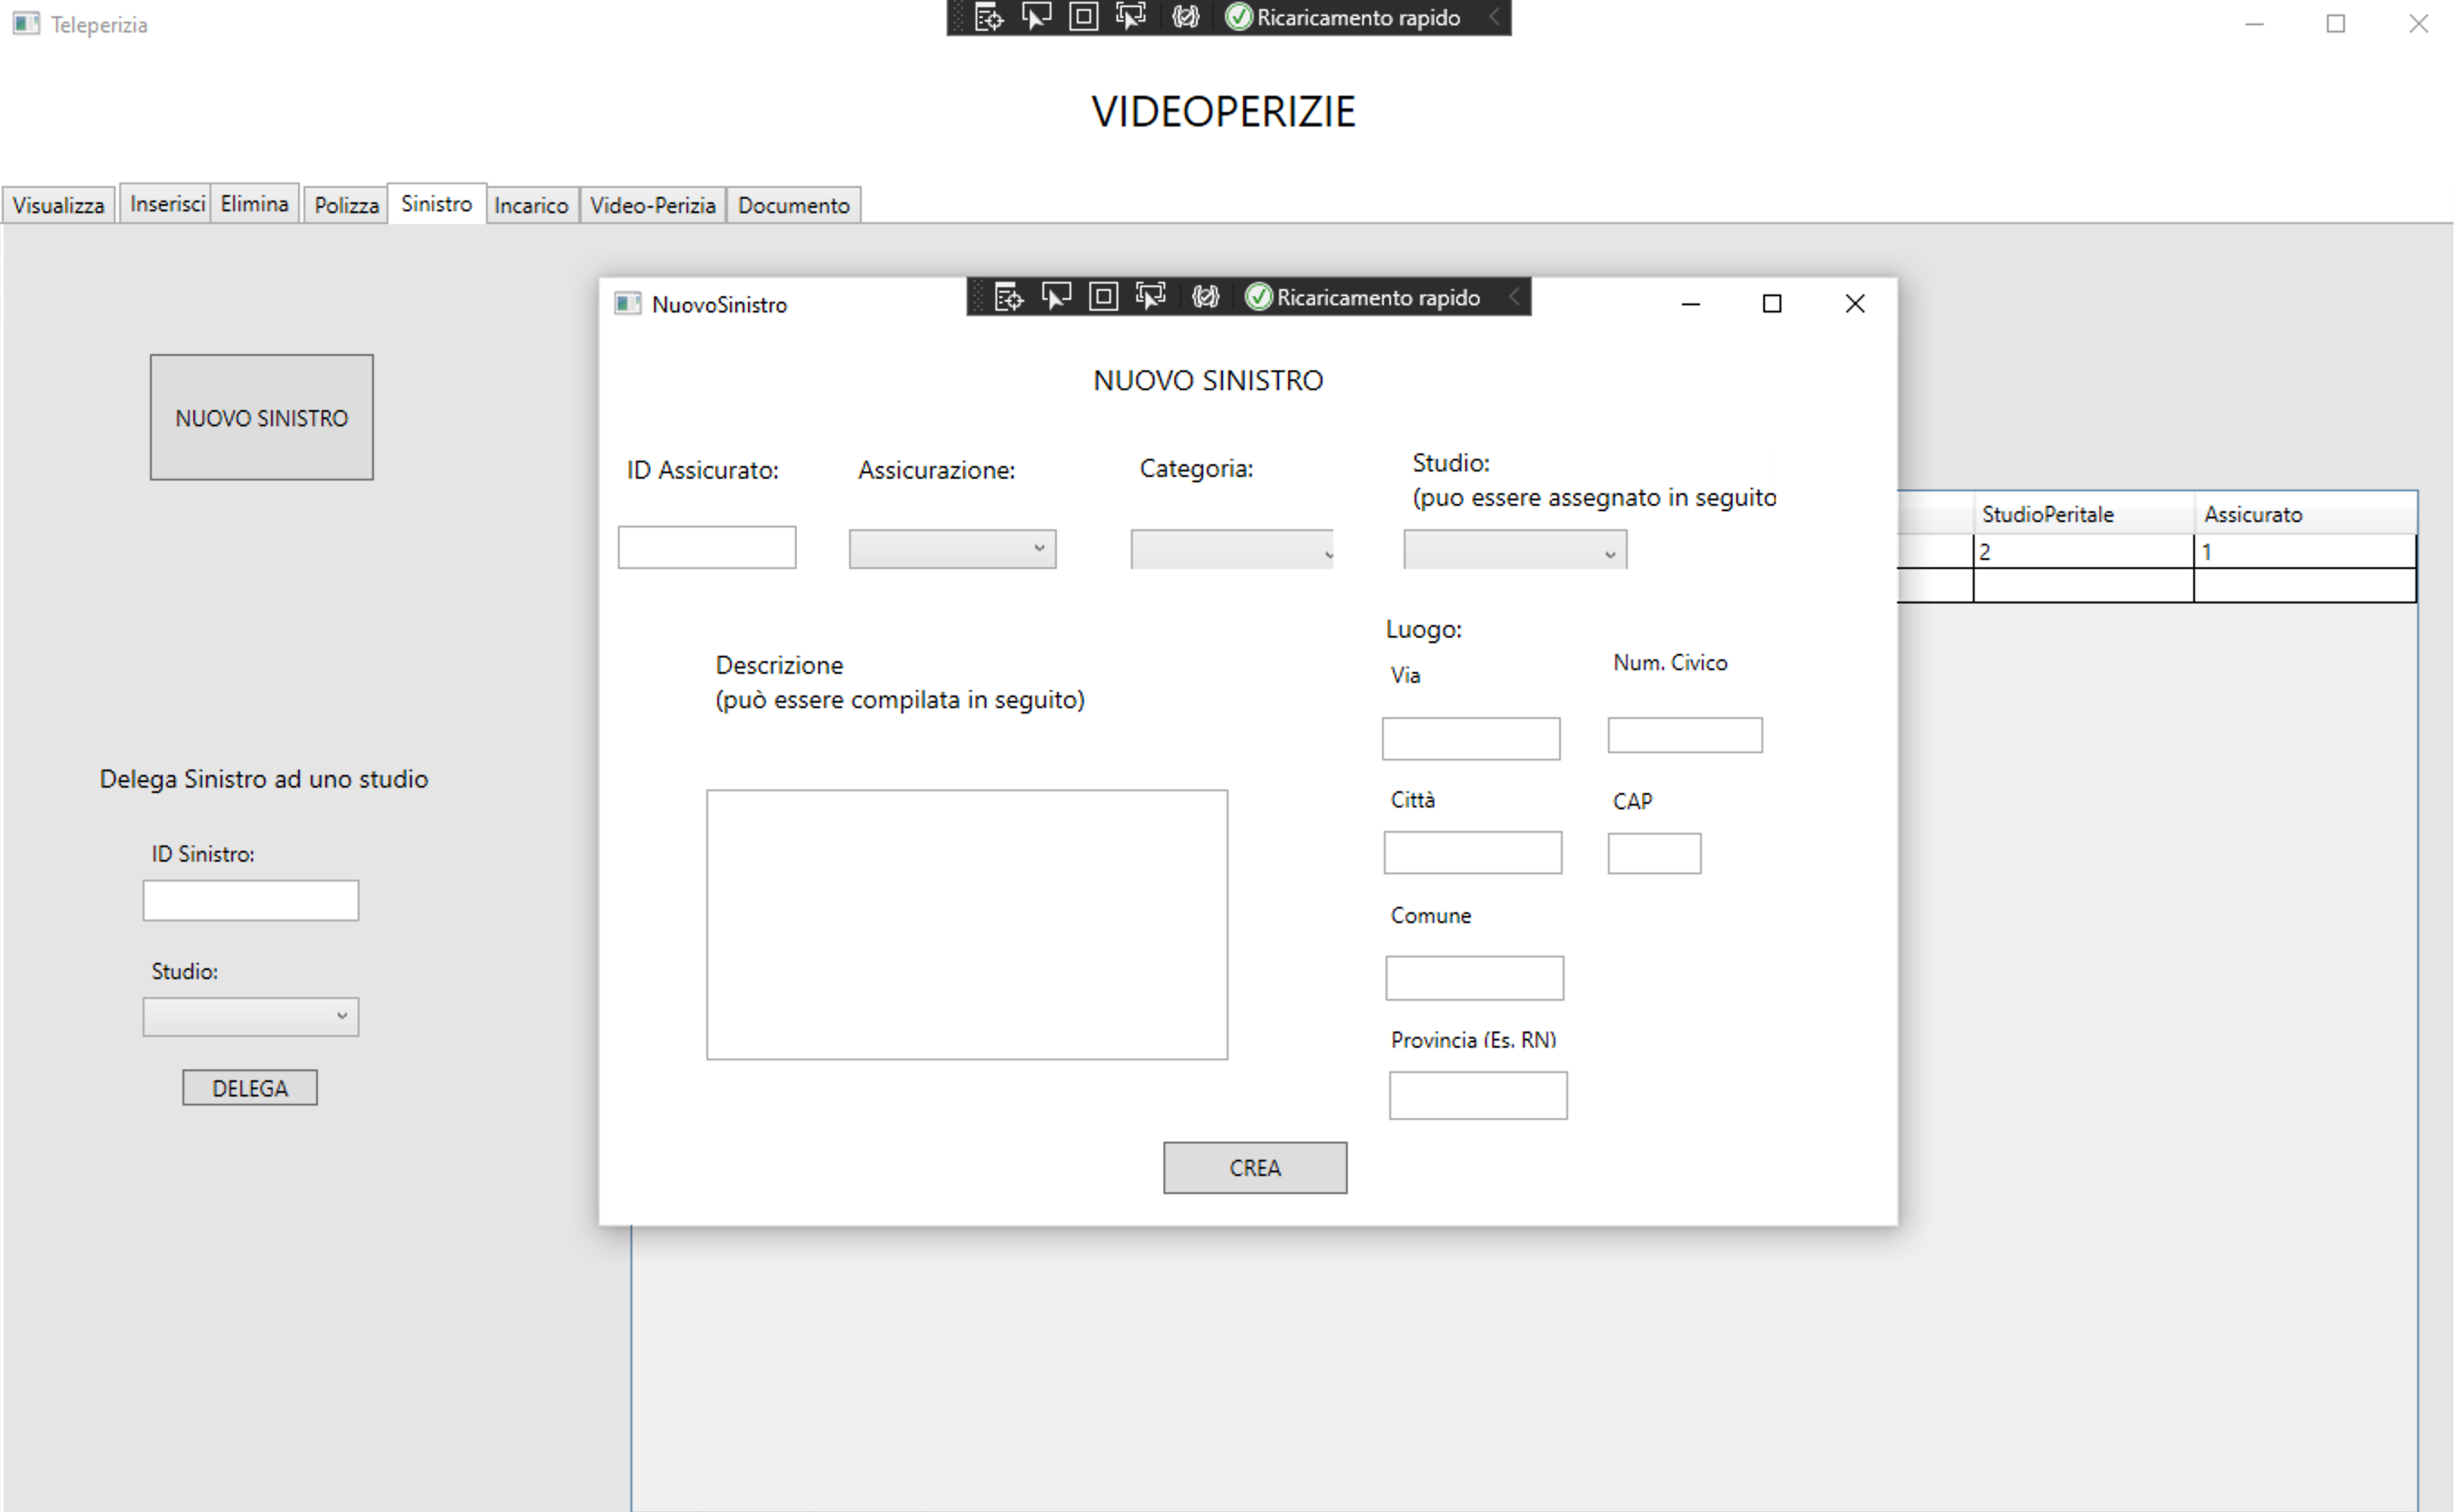
\includegraphics[width=\textwidth]{img/Applicazione/Sinistro2.png}
    \end{center}
\end{figure}
\clearpage
\section{Incarico}
Si possono creare e assegnare incarichi in un determinato studio, dando in input il supervisore il programma capisce automaticamente di che studio fa parte e propone i periti appartenenti a cui poter assegnare il nuovo incarico.

\begin{figure}[ht]
    \begin{center}
        \centering
        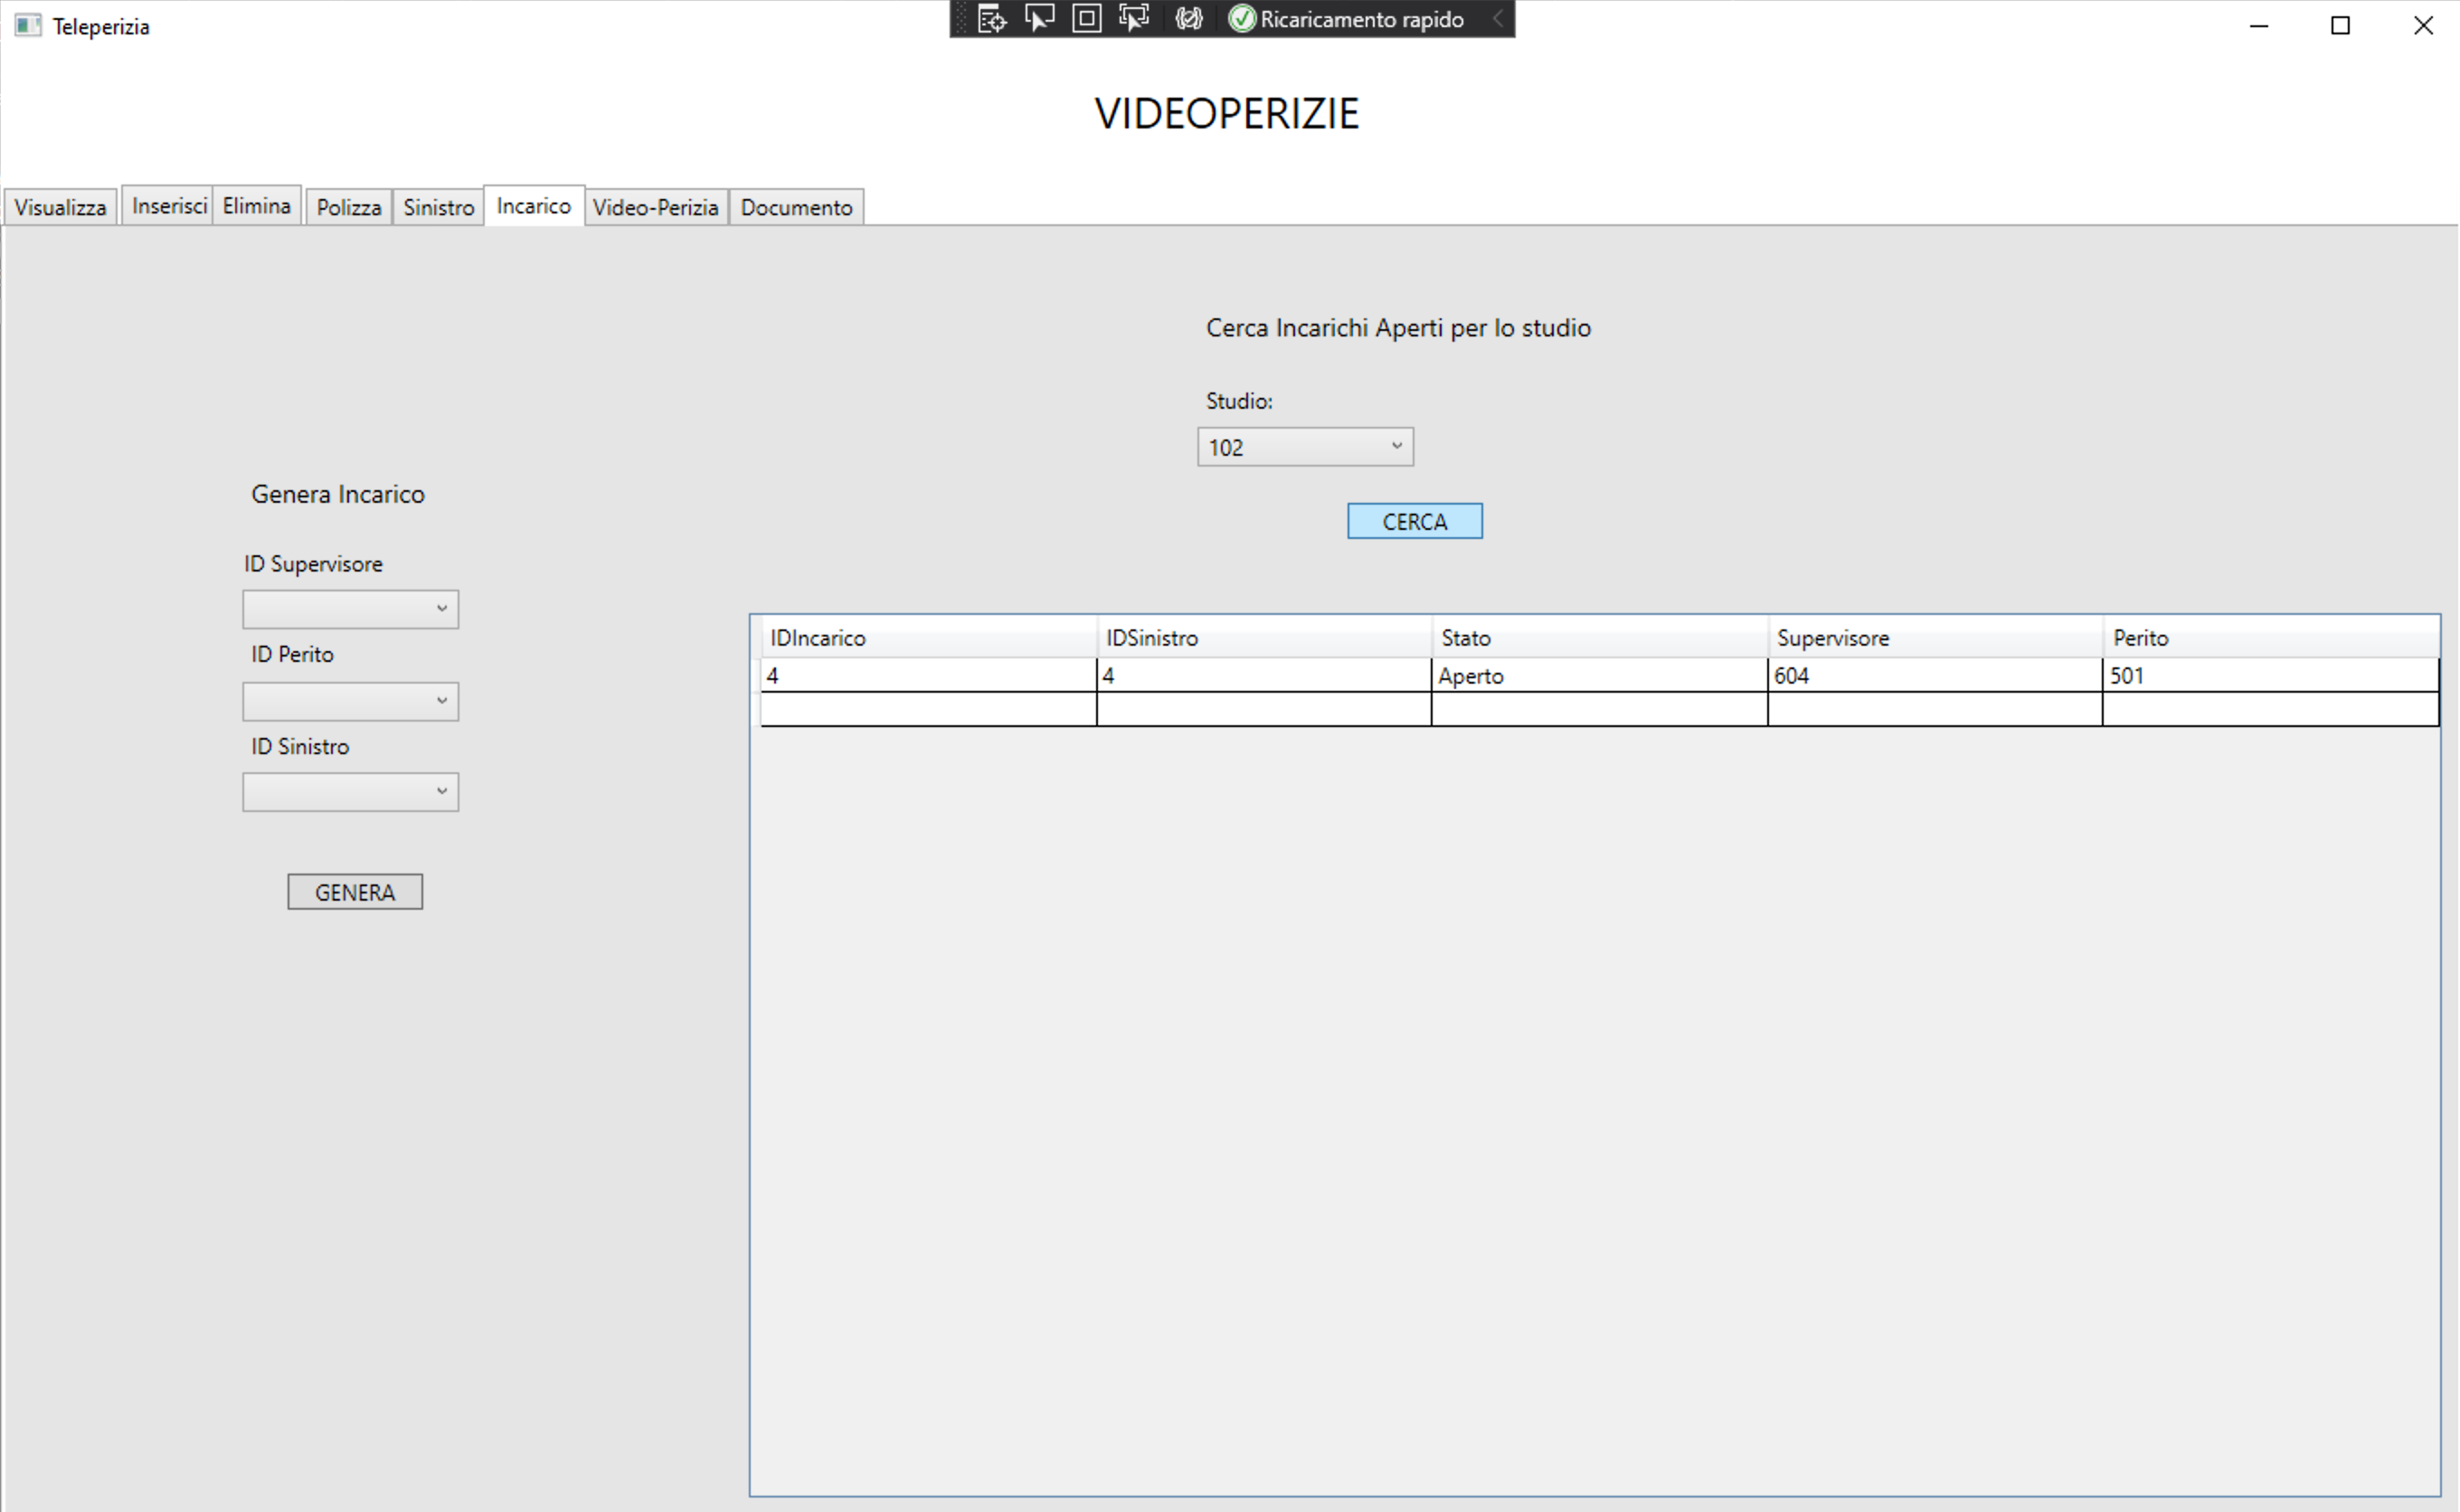
\includegraphics[width=\textwidth]{img/Applicazione/Incarichi.png}
    \end{center}
\end{figure}

\clearpage
\section{Video-perizia}
Si possono creare video-perizie, allegare media ad esse fornendo i dati giusti.

\begin{figure}[ht]
    \begin{center}
        \centering
        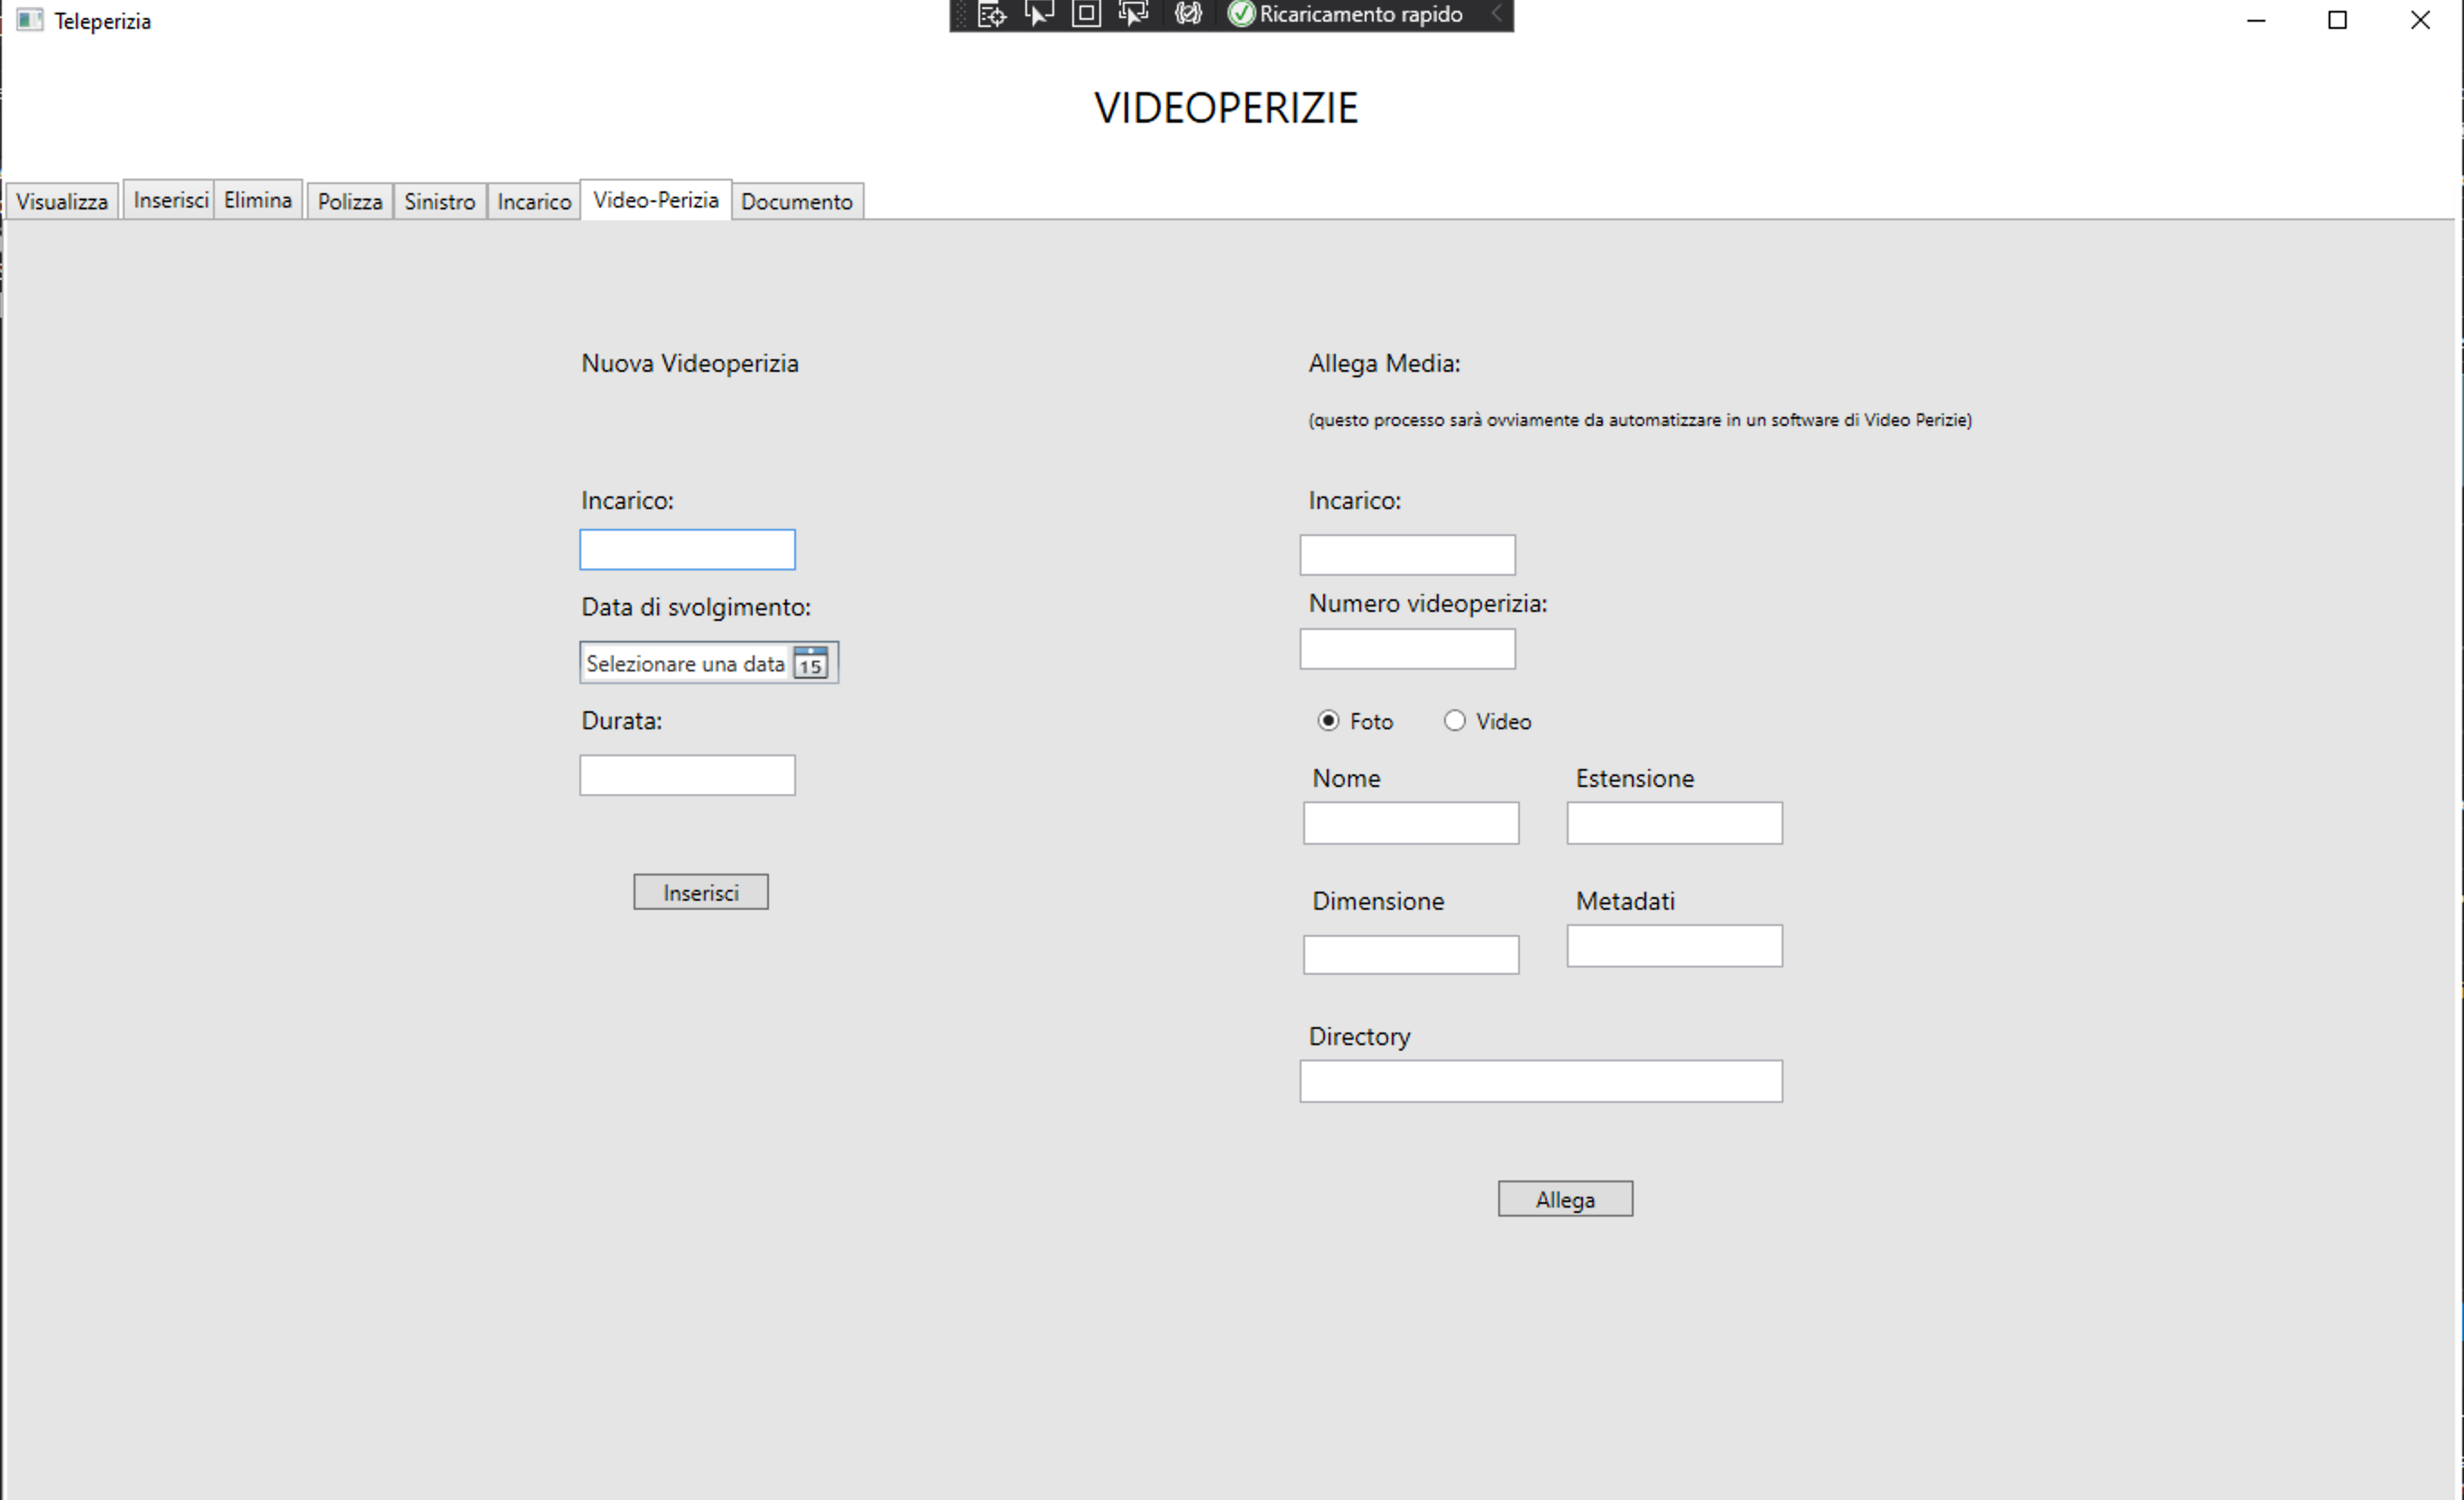
\includegraphics[width=\textwidth]{img/Applicazione/VideoPerizia.png}
    \end{center}
\end{figure}
\clearpage
\section{Documento}
Si possono allegare i documenti agli incarichi presenti nella base di dati.

\begin{figure}[ht]
    \begin{center}
        \centering
        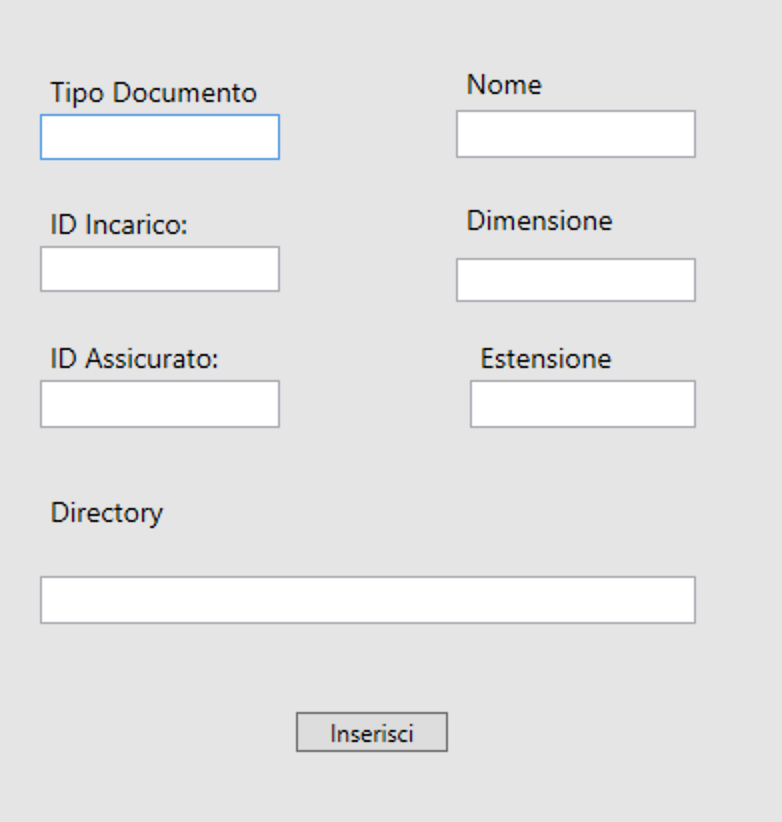
\includegraphics[scale=0.6]{img/Applicazione/Documento.png}
    \end{center}
\end{figure}

\end{document}
